\documentclass[final]{siamltex}
%test change
\usepackage{cite}
\usepackage{graphicx,bbm,pstricks,soul}
\usepackage{pifont}
\usepackage{bbm,algorithmic,mdframed,placeins,multirow,booktabs,subfigure}
\usepackage[ruled,vlined,linesnumbered]{algorithm2e}
\usepackage{tikz,hhline}
\usepackage{tabularx}
\newcolumntype{L}[1]{>{\raggedright\let\newline\\\arraybackslash\hspace{0pt}}m{#1}}
\newcolumntype{C}[1]{>{\centering\let\newline\\\arraybackslash\hspace{0pt}}m{#1}}
\newcolumntype{R}[1]{>{\raggedleft\let\newline\\\arraybackslash\hspace{0pt}}m{#1}}

\setlength{\parindent}{0in}
\usepackage{amsmath,amsfonts,amsbsy,amssymb}
\newcommand{\RARR}[3]{#1
  \;\displaystyle\mathop{\displaystyle\longrightarrow}^{#3}\; #2}
\newcommand{\RARRlong}[3]{#1
  \;\displaystyle\mathop{-\!\!\!-\!\!\!-\!\!\!-\!\!\!-\!\!\!\!\displaystyle
  \longrightarrow}^{#3}\; #2}
\newcommand{\LARR}[3]{#1
  \;\displaystyle\mathop{\displaystyle\longleftarrow}^{#3}\; #2}
\newcommand{\LRARR}[4]{{\mbox{ \raise 0.4 mm \hbox{$#1$}}} \;
  \mathop{\stackrel{\displaystyle\longrightarrow}\longleftarrow}^{#3}_{#4}
  \; {\mbox{\raise 0.4 mm\hbox{$#2$}}}}
\newcommand{\bX}{{\bf X}}
\newcommand{\vecx}{{\mathbf x}}
\newcommand{\vecy}{{\mathbf y}}
\newcommand{\vecz}{{\mathbf z}}
\newcommand{\vecq}{{\mathbf q}}
\newcommand{\bs}{{\mathbf s}}
\newcommand{\vecr}{{\mathbf r}}
\newcommand{\vecX}{{\mathbf X}}
\newcommand{\vecv}{{\mathbf v}}
\newcommand{\tick}{\ding{52}}
\newcommand{\cross}{\ding{54}}
\newcommand{\vecn}{{\mathbf n}}
\newcommand{\vecp}{{\mathbf p}}
\newcommand{\cT}{{\mathcal T}}
\newcommand{\dt}{{\mbox{d}t}}
\newcommand{\dx}{{\mbox{d} \vecx}}
\newcommand{\boldnu}{{\boldsymbol \nu}}
\newcommand{\er}{{\mathbb R}}
\renewcommand{\div}{{\rm div}}
\newcommand{\bnu}{{\bf \nu}}
\newcommand{\divergence}{\mathop{\mbox{div}}}
\renewcommand{\P}{\mathbb{P}}
\newcommand{\FP}{P_{\rm{FP}}}
\newcommand{\ME}{P_{\rm{ME}}}
\newcommand{\MEs}{P_{\rm{ME}_{S}}}
\newcommand{\D}{\mathcal{D}}
\newcommand{\G}{\mathcal{G}}
\newcommand{\N}{\mathcal{N}}
\newcommand{\X}{{\mathbf X}}
\newcommand{\Y}{{\mathbf Y}}
\newcommand{\W}{{\mathbf W}}
\newcommand{\data}{D}
\newcommand{\neff}{n_{\text{eff}}}
\newcommand{\E}{{\mathbb E}}
\renewcommand{\b}[1]{{\bf #1}}
\DeclareMathOperator*{\argmin}{arg\,min}
\DeclareMathOperator*{\argmax}{arg\,max}

\newcommand{\picturesAB}[6]{
\centerline{
\hskip #4
\raise #3 \hbox{\raise 0.9mm \hbox{(a)}}
\hskip #5
\epsfig{file=#1,height=#3}
\hskip #6
\raise #3 \hbox{\raise 0.9mm \hbox{(b)}}
\hskip #5
\epsfig{file=#2,height=#3}
}}
\newcommand{\picturesCD}[6]{
\centerline{
\hskip #4
\raise #3 \hbox{\raise 0.9mm \hbox{(c)}}
\hskip #5
\epsfig{file=#1,height=#3}
\hskip #6
\raise #3 \hbox{\raise 0.9mm \hbox{(d)}}
\hskip #5
\epsfig{file=#2,height=#3}
}}

\makeatletter  
\newcommand{\xleftrightarrows}[2][]{\mathrel{%  
 \raise.40ex\hbox{$  
       \ext@arrow 3095\leftarrowfill@{\phantom{#1}}{#2}$}%  
 \setbox0=\hbox{$\ext@arrow 0359\rightarrowfill@{#1}{\phantom{#2}}$}%  
 \kern-\wd0 \lower.4ex\box0}}  
 
\newcommand{\xrightleftarrows}[2][]{\mathrel{%  
 \raise.40ex\hbox{$\ext@arrow 3095\rightarrowfill@{\phantom{#1}}{#2}$}%  
 \setbox0=\hbox{$\ext@arrow 0359\leftarrowfill@{#1}{\phantom{#2}}$}%  
 \kern-\wd0 \lower.4ex\box0}}  
 
\def\leftrightarrowfill@{%
 \arrowfill@\leftarrow\relbar\rightarrow%
 }
\newcommand*{\centerfloat}{%
  \parindent \z@
  \leftskip \z@ \@plus 1fil \@minus \textwidth
  \rightskip\leftskip
  \parfillskip \z@skip}
\makeatother
\makeatother 

\newcommand\irregularcircle[2]{% radius, irregularity
  \pgfextra {\pgfmathsetmacro\len{(#1)+rand*(#2)}}
  +(0:\len pt)
  \foreach \a in {10,20,...,350}{
    \pgfextra {\pgfmathsetmacro\len{(#1)+rand*(#2)}}
    -- +(\a:\len pt)
  } -- cycle
}

\newcommand{\into}{\operatornamewithlimits{\longrightarrow}}
\newtheorem{dfn}{Definition}[section]

\newcommand{\ltri}{%
\,\resizebox{!}{0.25\baselineskip}{%
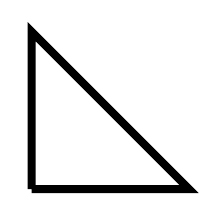
\begin{tikzpicture}%
\draw[line width=1mm](0,0) -- (0,2) -- (2,0)  -- (0,0);
\end{tikzpicture}%  
}\xspace%
}%

\newcommand{\smallltri}{%
\,\resizebox{!}{0.15\baselineskip}{%
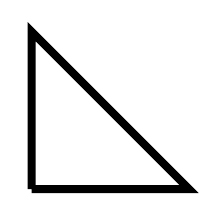
\begin{tikzpicture}%
\draw[line width=1mm](0,0) -- (0,2) -- (2,0)  -- (0,0);
\end{tikzpicture}%  
}\xspace%
}%

\author{Simon L. Cotter\thanks{School of
    Mathematics, University of Manchester, Manchester, UK. e:
    simon.cotter@manchester.ac.uk. SLC is grateful for EPSRC First
    grant award EP/L023393/1. SLC would like to thank the Isaac Newton
    Institute for Mathematical Sciences for support and hospitality
    during the programme ``Uncertainty quantification for complex systems: theory and methodologies'' when work on this paper was undertaken. This work was supported by:
EPSRC grant number EP/K032208/1.} \and Ioannis G. Kevrekidis\thanks{} \and Paul
  Russell\thanks{School of
    Mathematics, University of Manchester, Manchester, UK.}}

\title{Transport map accelerated adaptive importance sampling, and application to inverse problems arising from
  multiscale stochastic reaction networks}
\begin{document}
\maketitle
\begin{abstract}
In many applications, inverse problems arise where where there are
complex correlations between the different parameters which we wish to
infer from data. The correlations often manifest themselves as lower
dimensional manifolds on which the likelihood function is
invariant, or varies very little. This can be due to trying to infer
unobservable parameters, or due to sloppiness in the model which is
being used to describe the data. In such a situation, standard
sampling methods for characterising the posterior distribution which
do not incorporate information about this structure will be highly
inefficient. Moreover, most methods are inherently serial in nature,
and as such are not expoiting the parallelised  nature of modern
computer infrastructure. In this paper, we seek to develop a method to
tackle this problem, using optimal transport maps to simplify
posterior distributions which are concentrated on lower dimensional
manifolds.

We demonstrate the approach by considering inverse problems arising
from partially observed stochastic reaction networks. In particular,
we consider systems which exhibit multiscale behaviour, but for which
only the slow variables in the system are observable. We demonstrate
that certain multiscale approximations lead to more consistent
approximations of the posterior than others.
\end{abstract}


\section{Introduction}
%Topics to cover: parallel MCMC, pMC, PAIS
%Transport maps, transport map MCMC
%Stochastic reaction networks
%Multiscale approximations, QSSA/QEA, CMA

In Section \ref{sec:PAIS}, we will briefly reintroduce Parallel
Adaptive Importance Sampling (PAIS), a variant of Population Monte
Carlo (PMC) which incorporates state of the art resamplers. In Section \ref{sec:map} we show how an appropriate transport map can
be constructed from importance samples which maps the posterior close
to a reference Gaussian measure. In Section \ref{sec:TPAIS} we show
how such a map can be incorporated into a sophisticated parallel MCMC
infrastructure in order to accelerate mixing. In Section
\ref{sec:conv} we seek to show the advantages of this approach through
the analysis of a challenging test problem. In Section
\ref{sec:multi} we consider how likelihoods can be approximated using
 multiscale methodologies in order to carry out inference for
multiscale and/or partially observed stochastic reaction networks. In
Section \ref{sec:num} we present some numerical examples, which serve
to demonstrate the increased efficiency of the described sampling
methodologies, as well as investigating the posterior approximations
discussed in the previous section. We conclude with a discussion in
Section \ref{sec:conc}.

\section{Parallel Adaptive Importance Sampling}\label{sec:PAIS}
Parallel adaptive importance sampling (PAIS)\cite{cotter2015parallel} is a variant of PMC\cite{cappe2012population}, which is a family of methods which are based
on importance sampling. In importance sampling, we attempt to
characterise a target density through sampling from that
density. However, the target density $\pi$ itself is often too complex to sample
from directly, so we instead sample from a
proposal density $\chi$. Each sample $\theta^{(k)} \sim \chi$ is then weighted by
$w_k = \frac{\pi(\theta^{(k)})}{\chi(\theta^{(k)})}$, to take account of the bias of
sampling from a different distribution to $\pi$. Monte Carlo estimates
using a sample of size $N$
of a function $f$ with respect to $\pi$ can then be made through the
formula
\[\mathbb{E}_\pi(f) \approx \frac{1}{\bar{w}} \sum_{k=1}^N
  w_kf(\theta^(k)).\]
This method works well when $\pi$ and $\chi$ are close, but can be
excruciatingly slow when they are not. The idea behind PMC methods is
to construct a good proposal distribution, either from the entire
history of the algorithm up to the current point, or to use the
current state of a whole ensemble of $M$ particles in the system.

In PAIS, the proposal distribution $\chi$ is chosen to be the equally
weighted mixture of any choice of MCMC proposal kernel, evaluated at
each of the current particles in the system. If $\theta^{(k)} = [\theta_1^{(k)},
\theta_2^{(k)}, \ldots, \theta_M^{(k)}]^\top$ is the current state of the
ensemble, and we wish to use an MCMC proposal density $q(\cdot ;
\cdot, \beta)$ then 
\[\chi^{(k)} = \frac{1}{M} \sum_{i=1}^M q(\cdot ; \theta_i^{(k)}.\]
Often the variance of the MCMC proposal kernels can be tuned using
their respective algorithmic parameters $\beta$. Good values for these
algorithmic parameters can be
found by optimising for the effective sample size of the importance
sample that is produced (see \cite{cotter2015parallel, russ2017parallel} for more details).

If the ensemble is large enough, and the chain has entered
probabilistic stationarity, then the current state of the ensemble is
a good rough discrete approximation of the target density, and in turn
$\chi^{(k)}$ is close enough to $\pi$ to produce an efficient importance
sample $\{\hat{\theta}^{(k)},w^{(k)}\}$. It can be advantageous to use stratified sampling of the
mixture in order to
ensure that the sample made is as representative as possible of the
target density, i.e.
\[ \hat{\theta}_i^{(k)} \sim q(\cdot ; \theta_i^{(k)}\]
for each $i = 1,2,\ldots,M$. We now have a weighted sample, and it
would be inadvisable to use an equally weighted mixture of proposal
distributions from each of these points. Therefore, before starting
the next iteration, the importance sample
$\{\hat{\theta}^{(k)},w^{(k)}\}$ is resampled to produce an equally
weighted sample, ready for the next iteration of the algorithm. In
PAIS, a state-of-the-art resampler is used, which uses optimal
transport methods to find the equally weighted discrete sample which
best represents the statistics of the importance
sample\cite{reich2013nonparametric}. For larger ensemble sizes $M$ this can become
expensive, in which case a greedy approximation of this algorithm, the
Approximate Multinomial Resampler (AMR) can be
implemented\cite{cotter2015parallel}. The output of the resampler is then denoted
$\theta^{(k+1)}$ and the algorithm is ready for the next
iteration. The importance samples $\{\hat{\theta}^{(k)},w^{(k)}\}$ The PAIS is summarised in Algorithm \ref{alg:PAIS}.

\begin{table}[!h]
\centering
\begin{algorithm}[H]
\DontPrintSemicolon
\BlankLine
	Initialise $\theta^{(1)} \sim \mu_0$.\;
	\For{$k=1,\ldots,N$}{
		Sample $\hat{\theta}_i^{(k)} \sim q(\cdot; \theta_j^{(k)}, \beta)$, for $i = 1,\dots, M$.\label{algline:PAIS_propose}\;
		Calculate $w^{(k)} = (w_1^{(k)}, \ldots, w_M^{(k)})^\top$, where
			\[
				w^{(k)}_i = \frac{\mu(\hat{\theta}^{(k)}_i)}{\chi^{(k)}(\hat{\theta}^{(k)}_i; \theta^{(k)}, \beta)}.
			\]
		\label{algline:PAIS_weights}

		Resample $\theta^{(k+1)} \leftarrow \| w^{(k)}\|_1^{-1}\sum_{j=1}^M w_j^{(k)}\delta_{\hat{\theta}_j^{(k)}}(\cdot)$.\label{algline:PAIS_resample}\;
	}
	Output $\{(w^{(n)}, \hat{\theta}^{(n)}\}_{n=1}^N$.
\caption{The PAIS Algorithm.\label{alg:PAIS}}
\end{algorithm}
\end{table}

One problem with the PAIS and other PMC methods can become apparent if
the target density has very strong correlations in its structure, in
particular if that correlation is not global but only local. In this
case, unless the proposal densities $q$ are informed by this local
structure, the mixture distribution proposal may not well approximate
$\pi$ without a very large large ensemble size $M$, which can become
inhibitively expensive. Some methods have been
proposed\cite{douc2007minimum}
which use samples local to each particle to inform local covariance
structure.

In this paper, we investigate the use of transport maps to learn local
covariances across the whole of the domain, in order to stabilise
PMC-type methods, and make these methods more applicable to a wider
range of more challenging inference problems.

\section{Construction of transport maps in importance sampling} \label{sec:map}
%Follow the other papers, show adaptation(s)
In this Section, we describe the construction of transport maps which
allow for the simplification of complex posterior distributions in
order to allow for improved sampling, in particular for methods based
on importance sampling.
In~\cite{el2012bayesian} the transport map was introduced to provide a transformation from the prior
distribution to the posterior distribution, the idea being that one could draw a moderately sized
sample from the prior distribution and use this sample to approximate a map onto the target space.
Once this map was known to the desired accuracy a larger sample from the prior could be used to
investigate the posterior distribution. This
methodology was adapted in~\cite{parno2014transport} to form a new proposal method for MH
algorithms. In this case, rather than transforming a sample from the prior into a sample from the target
distribution, the map transforms a sample from the posterior onto a reference space.
The reference density is chosen to allow efficient proposals using a simple proposal
distribution such as a Gaussian centred at the previous state. Proposed states can then be mapped back into a sample from the posterior by applying the inverse of the transport map.

Proposing new states in this way allows us to make large steps around complex probability distributions.
It is also feasible in this framework to assume that the reference density is close enough to a standard Gaussian that we can efficiently propose moves using a proposal distribution which is independent of the current state, e.g. choose $q(\theta) = \mathcal{N}(0,I_n)$.

In this Section we outline the methodology in
\cite{parno2014transport} for approximately coupling the target,
$\mu_{\theta}$, with the reference distribution, $\mu_r$, and
show how the map can be constructed using a weighted sample
and hence how we can incorporate the map into importance sampling schemes.

\begin{dfn}[Transport Map $T$]
	A transport map $T$ is a function $T\colon
        \mathcal{X}\rightarrow\mathbb{R}^d$ such that the {\it
          pullback} of the reference measure with density $\phi(\cdot)$,
	\begin{equation}\label{eq:pullback}
		\tilde{\pi}(\theta) = \phi(T(\theta))|J_T(\theta)|,
	\end{equation}
	is equal to the target density $\pi(\theta)$ for all $\theta \in \mathcal{X}$. The pullback is defined in terms of the determinant of the Jacobian of $T$,
	\[
		|J_T(\theta)| = \text{det}\begin{bmatrix} \partial_{\theta_1} T_1(\theta) & \dots & \partial_{\theta_d} T_1(\theta) \\ \vdots & \ddots & \vdots \\ \partial_{\theta_1} T_d(\theta) & \dots & \partial_{\theta_d} T_d(\theta) \end{bmatrix}.
	\]
\end{dfn}

% In the case that we have an invertible map,
% $T\in\mathcal{T}$ where $\mathcal{T}$ is the space of all invertible
% maps, we are able to draw a sample from $\pi_r = \phi$, the density of
% the reference distribution, which could be picked to be the
% standardised Gaussian distribution for example, and map these samples back
% onto target space using $T^{-1}$. These proposed samples are then distributed according to the target distribution.

\begin{dfn}[Target and Reference Space]
	The transport map pushes a particle from a {\it target space} $\mathcal{X}$, that is a subset of $\mathbb{R}^d$ equipped with a target measure $\mu_{\theta}$, onto a {\it reference space}, $R$, again a subset of $\mathbb{R}^d$ equipped with the reference measure $\mu_r$.
\end{dfn}

Armed with such a map, independent samples can be made of the target
measure, using the pullback of the reference density $\phi$ through $T^{-1}$.
Clearly the pullback only exists when $T$ is monotonic, i.e. has a positive definite Jacobian, and has continuous first derivatives.
Not all maps satisfy these conditions, so we define a smaller space of
maps, $\mathcal{T}^\uparrow \subset \mathcal{T}$ which contains all
feasible maps. This space does not necessarily contain an exact
coupling between target and reference space, and so we are motivated to formulate an optimisation problem to find the map $\tilde{T}
\in \mathcal{T}^\uparrow$ which most closely maps the target density
to the reference density.

% We attempt to find the deterministic coupling of two continuous
% probability distributions, $(\mu_\theta, \hat{\mu_r})$, such that
% $\hat{\mu_r} = T\mu_\theta$ where the distance between $\mu_r$ (the
% desired reference measure) and $\hat{\mu_r}$ (the achieved reference
% measure) is minimised, for $T \in \mathcal{T}^\uparrow$. As in
% \cite{parno2014transport} we aim to minimise the Kullback-Liebler (KL)
% divergence between the density of $\mu_{\theta}$ and the pullback of
% the density of $\mu_{r}$, i.e. the distance between $\pi(\theta)$ and
% $\tilde{\pi}(\theta)$. For two absolutely continuous measures with
% densities $\pi_1$ and $\pi_2$ respectively, the KL
% divergence is given by
% \[D_\text{KL}(\pi_1\|\pi_2) = 
% 		\mathbb{E}_{\pi_1}\left[\log\left(\frac{\pi_1(\theta)}{\pi_2(\theta)}\right)\right].\]
% The KL divergence is not itself a norm, since
% it is not symmetric, i.e. $D_\text{KL}(\pi_1\|\pi_2) \neq
% D_\text{KL}(\pi_2\|\pi_1)$ in general. However, it is still a useful
% measure of the similarity of two probability distributions, not least since the
% square root of the KL-divergence is an upperbound to the Hellinger
% distance metric.

As in previous work in \cite{parno2014transport}, we can ensure
invertibility if we restrict the map to be lower triangular, i.e. $\tilde{T} \in \mathcal{T}^{\ltri}\subset\mathcal{T}^\uparrow$. This lower triangular map has the form,
\[
	T(\theta_1, \dots, \theta_n) = \begin{bmatrix} T_1(\theta_1) \\ T_2(\theta_1, \theta_2) \\ \vdots \\
		T_n(\theta_1, \dots, \theta_n) \end{bmatrix},
\]
where $T_i\colon \mathbb{R}^i \to \mathbb{R}$. % We assume that the target and reference probability densities are absolutely continuous on
% $\mathbb{R}^d$. Under this formulation, with appropriate
% regularisation (which will be detailed later), we are guaranteed a unique invertible map $\tilde{T}$ with the property that
% \[
% 	\tilde{T}\mu_{\theta} \approx \mu_r.
% \]
% % Relaxing the equality constraint to finding the approximate map
% % $\tilde{T} \in \mathcal{T}^{\ltri}$ which minimises $C(T)$, gives us a
% % practical route to finding a good candidate map.

\subsection{The optimisation problem}
Our aim is now to find the lower triangular map $\tilde{T} \in
\mathcal{T}^{\ltri}$ such that the difference between target
density and the pullback of the reference density is minimised. As in
\cite{parno2014transport}, we choose the cost function
to be the Kullback-Leibler (KL) divergence between the posterior density and the pullback density,
\[
	D_\text{KL}(\pi\|\tilde{\pi}) =
		\mathbb{E}_\pi\left[\log\left(\frac{\pi(\theta)}{\tilde{\pi}(\theta)}\right)\right].
\]
This divergence results in some nice properties which we will explore in the following derivation. The KL divergence is not a true metric since it is not symmetric, however it is commonly used to measure the distance between probability distributions due to it's relatively simple form, and because it provides a bound for the square of the Hellinger distance by Pinsker's inequality~\cite{pinsker1960information},
\[
	D_{KL}(p\|q) \geq D_H^2(p,q),
\]
which is a true metric between probability distributions $p$ and $q$.
Given the form of the pullback in Equation~\eqref{eq:pullback}, now taken through an approximate map $\tilde{T}$, the divergence becomes
\[
	D_\text{KL}(\pi\|\tilde{\pi}) = \mathbb{E}_\pi\left[\log\pi(\theta) - \log\pi_r(\tilde{T}(\theta)) -
		\log\left|J_{\tilde{T}}(\theta)\right|\right].
\]
We note the posterior density is independent of $\tilde{T}$, and so it is not necessary for us to compute it when optimising this cost function. This expression is a complicated integral with respect to the target distribution, for which the normalisation constant is unknown. However this is exactly the scenario for which we would turn to MCMC methods for a solution.

To find the best coupling, $\tilde{T} \in \mathcal{T}^{\ltri}$, we solve the optimisation problem,
\[
	\tilde{T} = \arg\min_{T \in \mathcal{T}^{\smallltri}} \mathbb{E}_\pi\left[-\log\pi_r(T(\theta)) -
		\log\left|J_T(\theta)\right|\right]
\]
which has a unique solution since the cost function is convex. We also include a regularisation term, which is required for reasons which will become clear later. The optimisation problem now takes the form
\begin{equation}\label{eq:gen_map_optim}
	\tilde{T} = \arg\min_{T\in\mathcal{T}^{\smallltri}} \left[
		 \mathbb{E}_\pi\left[-\log\pi_r(T(\theta)) -
		\log\left|J_T(\theta)\right|\right] + \beta\mathbb{E}(T(\theta)- \theta)^2 \right].
\end{equation}
The parameter $\beta>0$ does not need to be tuned, as experimentation has shown that the choice
$\beta=1$ is sufficient for most problems. This expectation can be
approximated by using an MCMC approximation. The form of the penalisation term promotes maps which are
closer to the identity, and so prevents overfitting when the quality
or size of the current sample from the posterior is not sufficient.

\subsection{The structure of the map}

Before we continue with the derivation of the optimisation problem, we consider the structure
of the map in more detail. The lower triangular structure of the map not only guarantees monotonicity, it also allows for efficient calculation of the pullback density, as well as the inverse of the map, $\tilde{T}^{-1}$. The Jacobian of $\tilde{T}$ is a lower triangular matrix,
\[
	J_T(\theta) = \begin{bmatrix}
		\partial_{\theta_1} \tilde{T}_1(\theta) & \dots & \partial_{\theta_d} \tilde{T}_1(\theta)\\
		\vdots & \ddots & \vdots \\
		\partial_{\theta_1} \tilde{T}_d(\theta) & \dots & \partial_{\theta_d} \tilde{T}_d(\theta)
	\end{bmatrix} = \begin{bmatrix}
		\partial_{\theta_1} \tilde{T}_1(\theta) & \dots & 0\\
		\vdots & \ddots & \vdots \\
		\partial_{\theta_1} \tilde{T}_d(\theta) & \dots & \partial_{\theta_d} \tilde{T}_d(\theta)
	\end{bmatrix}
\]
since $\partial_{\theta_n} \tilde{T}_k(\theta) = 0$ for all $n > k$. This lower triangular structure means that the determinant of the Jacobian is a product of the diagonal elements which, when we take logs, becomes
\begin{equation}\label{eqn:separable_jacobian}
	\log\left|J_{\tilde{T}}(\theta)\right| = \sum\limits_{i=1}^d \! \log \partial_{\theta_i} \tilde{T}_i(\theta),
\end{equation}
where we note that this term is separable in terms of the dimension $i$.

Inverting $\tilde{T}$ at a point $r$ is simplified by the lower triangular structure of the map. The map component $\tilde{T}_1(\theta)$ is a univariate polynomial in $\theta_1$, so we can find the inverse of this function by solving the equation $T_1(\theta_1) = r_1$. This inversion tells us the value of $\theta_1$, which means the next component is again a univariate polynomial, $T_2(\theta_2; \theta_1)=r_2$. We can then perform $d$ root finding problems instead of a full $d$ dimensional non-linear solve.

We require that the first derivatives of the map are continuous, which is easy to enforce by the choice of basis functions. Here we assume that the map will be built from a family of orthogonal polynomials, $\mathcal{P}(\theta)$, not necessarily orthogonal with respect to the target distribution. Each component of the map is defined as a multivariate polynomial expansion,
\begin{equation}\label{eq:map_defn}
	\tilde{T}_i(\theta; \gamma_i) = \sum\limits_{\mathbf{j}\in\mathcal{J}_i} \!
\gamma_{i,\mathbf{j}}\psi_\mathbf{j}(\theta).
\end{equation}
The parameter $\gamma_i \in \mathbb{R}^{M_i}$ is a vector of coefficients. Each component of $\gamma_i$ corresponds to a basis function
$\psi_\mathbf{j}$, indexed by the multi-index $\mathbf{j} \in \mathbb{N}_0^d$. These multi-indices are elements of the multi-index set $\mathcal{J}_i$. A multi-index defines a product of univariate polynomials in $\theta_k$,
\[
	\psi_\mathbf{j}(\theta) = \prod\limits_{k=1}^i \! \varphi_{j_k}(\theta_k), \quad \text{for} \quad \mathbf{j} \in \mathcal{J}_i,
\]
and where $\varphi_{j_k}(\theta_k) \in \mathcal{P}(\theta_k)$. Since $\tilde{T}$ is lower triangular, a multi-index $\mathbf{j}\in\mathcal{J}_i$ only contains entries for univariate polynomials in $\theta_k$ for $k\leq i$.

The cardinalities of the multi-index sets, $M_i = \text{card}(\mathcal{J}_i)$, give the number of unknowns in our
optimisation problem, and so we would like to keep this number as small as possible. One option is
to use polynomials of total order $p$,
\[
	\mathcal{J}_i^\text{TO} = \left\{\mathbf{j}:\|\mathbf{j}\|_1 \leq p, j_k = 0\ \forall k > i\right\},
\]
which is optimal in terms of the amount of information captured by the map about the target. The cardinality of $\mathcal{J}_i^\text{TO}$ is $M_i = \binom{i+p}{p}$ which increases rapidly in $d$ and $p$, where $i = 1, \dots, d$. Smaller optimisation problems can be produced by constructing subsets of $\mathcal{J}_i^\text{TO}$. These index sets are discussed
in~\cite{parno2014transport}. Increased information with a slower increase in the number of map parameters can be achieved with the composition of maps discussed in~\cite{parno2015transport}. Here we stick with polynomials of total order $p$ since we work with low dimensional problems with the PAIS algorithm.


\subsection{Implementation of the optimisation problem}\label{sec:transport_implementation}

We now discuss how we can evaluate the cost function in
Equation~\eqref{eq:gen_map_optim}. In \cite{parno2014transport}, this
expectation is approximated using an MCMC estimator, such that
\begin{align}
	C(T) &= \mathbb{E}_\pi\left[ -\log\pi_r(T(\theta)) - \log|J_T(\theta)|\right] +
			\beta\mathbb{E}(T(\theta)-\theta)^2 \notag \\
		&\approx \frac{1}{K}\sum\limits_{i=1}^d \! \sum\limits_{k=1}^K \left[-\log\pi_r(T_i(\theta^{(k)})) -
			\log\left|\frac{\partial T_i}{\partial \theta_i}(\theta^{(k)})\right| + \beta(T_i(\theta^{(k)})-\theta^{(k)})^2\right]. 
\end{align}
Here we diverge from previous work, as we aim to build a map from
samples from an importance sampling scheme. Such samples no longer
carry equal weight, and as such the Monte Carlo estimator becomes
\begin{equation}\label{eqn:TM_full_cost}
	C(T) = \frac{1}{\bar{w}}\sum\limits_{i=1}^d \! \sum\limits_{k=1}^K
		w_k \left[-\log\pi_r(T_i(\theta^{(k)})) -
			\log\left|\frac{\partial T_i}{\partial \theta_i}(\theta^{(k)})\right| + \beta(T_i(\theta^{(k)})-\theta^{(k)})^2\right],
\end{equation}
where $w_k$ are the weights associated with each sample $\theta^{(k)}$, and $\bar{w}$ is the sum of
all these weights. Optimisation of this cost function results in a map from $\pi$ to some reference density $\pi_r$. By choosing the reference density to be a Gaussian density, we can simplify this expression greatly. Substitution of the Gaussian density into Equation~\eqref{eqn:TM_full_cost} leads to
\begin{equation}\label{eqn:TPAIS_objective}
	C(T) = \frac{1}{\bar{w}}\sum\limits_{i=1}^d \! \sum\limits_{k=1}^K
		w_k\left[\frac{1}{2}T_i^2(\theta^{(k)}) - \log\frac{\partial
		T_i}{\partial\theta_i}(\theta^{(k)}) + \beta(T_i(\theta^{(k)})-\theta^{(k)})^2\right],
\end{equation}

Note that since we assume that the map is monotonic, the derivatives of each component are
positive and so this functional is always finite. In practice it is infeasible to enforce this condition across the whole parameter space. We instead enforce this condition by ensuring that the derivatives are positive at each sample point. This means that when we sample away from these support points while in reference space, it is possible to enter a region of space where the map is not monotonic.

We now return to the structure of the map components given in Equation~\eqref{eq:map_defn}. Since the basis functions are
fixed, the optimisation problem in \eqref{eq:gen_map_optim} is really over the map components $\bar{\gamma} = (\gamma_1, \dots,
\gamma_d)$ where $\gamma_i \in \mathbb{R}^{M_i}$. Note that $C(T)$ is the sum of $d$ expectations, and these expectations each only concern one dimension. Therefore we can rewrite \eqref{eq:gen_map_optim} as $d$ separable optimisation problems.
\begin{align}\label{eq:gamma_map_optim}
	&\arg\min_{\gamma_i\in\mathbb{R}^{M_i}} \frac{1}{\bar{w}}\sum\limits_{k=1}^K
		w_k \left[\frac{1}{2}T_i^2(\theta^{(k)}; \gamma_i) - \log\frac{\partial T_i}{\partial\theta_i}(\theta^{(k)}; \gamma_i) + \beta(T_i(\theta^{(k)};
		\gamma_i)-\theta^{(k)})^2\right], \\
	&\text{subject to} \quad \frac{\partial T_i}{\partial\theta_i}(\theta^{(k)};
		\gamma_i) > 0 \ \text{for all}\ k=1,\dots,K,\ i=1,\dots,d.
		\notag
\end{align}
The sum in Equation~\eqref{eq:map_defn} is an inner
product between the vector of map coefficients, and the evaluations of the basis function at a
particular $\theta^{(k)}$. If we organise our basis evaluations into two matrices,
\[
	(F_i)_{k,\mathbf{j}} = \psi_\mathbf{j}(\theta^{(k)}), \quad \text{and} \quad (G_i)_{k,\mathbf{j}} =
\frac{\partial\psi_\mathbf{j}}{\partial\theta_i}(\theta^{(k)}),
\]
for all $\mathbf{j}
\in \mathcal{J}_i^\text{TO}$, and $k = 1,\dots,K$, then we have that
\[
	T_i(\theta^{(k)}) = (F_i)_{k\cdot}\gamma_i \quad \text{and} \quad \frac{\partial T_i}{\partial \theta_i}(\theta^{(k)}; \gamma_i) = (G_i)_{k\cdot}\gamma_i,
\]
so \eqref{eq:gamma_map_optim} becomes
\begin{align}\label{eq:blas_map_optim}
	&\arg\min_{\gamma_i\in\mathbb{R}^{M_i}}
          \frac{1}{2}(F_i\gamma_i)^\top W (F_i\gamma_i) -
		{\bf w}^\top\log(G_i\gamma_i) + \frac{\beta}{\bar{w}}\sum\limits_{k=1}^K \!
		w_k(F_i\gamma_i-\theta^{(k)})^\top(F_i\gamma_i-\theta^{(k)}), \\
	&\text{subject to} \quad G_i\gamma_i > 0. \notag
\end{align}
In this expression, the vector ${\bf w} = [w_1, w_2, \ldots,
w_K]^\top$ is the vector of the weights, $W$ is the diagonal matrix $W
= \text{diag}(w)$ and $\log(G_i\gamma_i)$ is to be
evaluated element-wise. As more importance samples are made, new rows can be appended to the
$F_i$ and $G_i$ matrices, and $F_i^\top W F_i$ can be efficiently updated via the addition of rank-1 matrices.

The regularisation term in Equation~\eqref{eq:blas_map_optim} can be approximated using Parseval's identity,
\[
	\frac{1}{\bar{w}}\sum\limits_{k=1}^K \! w_k
        (F_i\gamma_i-\theta^{(k)})^\top(F_i\gamma_i-\theta^{(k)})
        \xrightarrow[K \to \infty]{}
		\int_{\mathbb{R}^n} |T(\theta)-\theta|^2 \text{d}\mu_\theta =
		\sum\limits_{\mathbf{j}\in\mathcal{J}_i^\text{TO}} (\gamma_{i,\mathbf{j}}-\iota_\mathbf{j})^2,
\]
where $\iota$ is the vector of coefficients for the identity map. This is of course only true when
the polynomial family $\mathcal{P}(\theta)$ is chosen to be orthonormal with respect to $\mu_\theta$; however this
approximation prevents the map from collapsing onto a Dirac when the expectation is badly approximated by a small number of samples.% If we do not normalise the MC estimator by $K$, we can allow this regularisation term to be dominated by the rest of the cost function as $K$ increases.

These simplifications result in the efficiently implementable, regularised optimisation problem for
computing the map coefficients, 
\begin{align}\label{eq:weighted_map_optim}
	&\arg\min_{\gamma_i\in\mathbb{R}^{M_i}} \frac{1}{2\bar{w}}\gamma_i^\top F_i^\top WF_i\gamma_i -
		\frac{w^\top}{\bar{w}}\log(G_i\gamma_i) + \beta\|\gamma_i-\iota\|^2, \\
	&\text{subject to} \quad G_i\gamma_i > 0, \notag
\end{align}
%where additionally we have introduced a factor of $\frac{1}{K}$ to the
%regularisation term to prevent over-smoothing as the number of samples increases.
This optimisation problem can be efficiently solved using Newton iterations. It is suggested
in~\cite{parno2014transport} that this method usually converges in around 10-15 iterations, and we
have seen no evidence that this is not a reasonable estimate. When calculating the map several times
during a Monte Carlo run, using previous guesses of the optimal map to seed the Newton algorithm
results in much faster convergence, usually taking only a couple of iterations to satisfy the stopping
criteria.

The Hessian takes the
form
\begin{equation}\label{eqn:TPAIS_hessian}
	HC_i(\gamma_i) = \frac{1}{\bar{w}}\left[F_i^\top WF_i + G_i^\top
		W\text{diag}([G_i\gamma_i]^{-2})G_i\right] + \beta I,
\end{equation}
where $[G_i\gamma_i]^{-2}$ is to be taken element-wise, and $I$ is the $M_i\times M_i$
identity matrix. The first derivative of $C_i(T)$ is
\[
	\nabla C_i(\gamma_i) = \frac{1}{\bar{w}}\left[F_i^\top WF_i\gamma_i - G_i^\top
		W[G_i\gamma_i]^{-1}\right] + \beta(\gamma_i - \iota),
\]
again $[G_i\gamma_i]^{-1}$ is taken element-wise.



\section[Transport map MCMC]{Transport map usage in PAIS
  and other PMC algorithms}\label{sec:TPAIS}

Given importance samples from the target distribution, we have demonstrated how to construct an approximate transport map from the
target measure to a reference measure. We now consider how to
implement an importance sampling-based MCMC algorithm which uses
these maps to propose new states. In \cite{parno2014transport} it was
shown how approximate transport maps can be used to accelerate
Metropolis-Hastings methods, with the map being periodically updated
with the samples produced from the target measure. Convergence of this
adaptation is shown in~\cite{parno2014transport}. In this Section, we
will show how similarly, these maps can be used to construct highly
efficient importance sampling schemes.

In particular, we will show how we can use the transport map derived in Equation~\eqref{eq:weighted_map_optim} to
design a proposal scheme for the PAIS algorithm. In this case we have a choice in how to proceed; we
propose new samples on reference space and resample on target space, or we both propose and resample on reference space, mapping onto target space to output the samples. The first option allows us to reuse much of the framework
from the standard PAIS algorithm and in the numerics later we see that this performs better than
both the Transport MH algorithm, and the standard PAIS algorithm. The second option requires some
restructuring but results in improved performance from the resampler.

\begin{table}
\begin{algorithm}[H]
\DontPrintSemicolon
\BlankLine
Initialise state $\theta^{(1)}_i = \theta_0$, \quad $i = 1,\dots,M$.\;
Initialise map $\bar{\gamma}^{(1)} = \iota$.\;
\For{$k \leftarrow 1, \dots, L-1$}{
	Compute $r_i = \tilde{T}(\theta^{(k)}_i; \bar{\gamma}^{(k)})$, \quad $i = 1,\dots,M$.\;
	Sample $r'_i \sim q_r(\cdot; r_i)$.\;
	Invert $\hat{\theta}_i^{(k)} = \tilde{T}^{-1}(r'_i; \bar{\gamma}^{(k)})$.\;
	Calculate:
	\[
		w_i^{(k)} = \frac{\pi(\hat{\theta}_i^{(k)})}{\left(\sum_{j=1}^M \! q_r(r_i'; r_j)\right)|J_{\tilde{T}}(\hat{\theta}_i^{(k)};\bar{\gamma}^{(k)})|}.
	\]

	Resample $\theta^{(k+1)} \leftarrow \|w^{(k)}\|^{-1}\sum\limits_{j=1}^M \! w_j^{(k)}\delta_{\hat{\theta}^{(k)}_j}(\cdot)$.\;

	\eIf{$k\ \text{mod}\ K_U = 0$ and $k < K_\text{stop}$}{
		\For{$i \leftarrow 1, \dots, n$}{
			Solve \eqref{eq:weighted_map_optim} with $\{(w^{(1)},\hat{\theta}^{(1)}), \dots, (w^{(k+1)},\hat{\theta}^{(k+1)})\}$
				and update $\gamma_i^{(k+1)}$.\;
		}
	}{
		$\bar{\gamma}^{(k+1)} = \bar{\gamma}^{(k)}$.\;
	}
}
\caption{PAIS algorithm with adaptive transport map. Option 1.\label{alg:TransportPAIS1}}
\end{algorithm}
\end{table}

The first option is given in Algorithm~\ref{alg:TransportPAIS1}. We
denote the ensembles of states in target space $\theta^{(k)} =
\{\theta^{(k)}_1,\dots,\theta^{(k)}_M\}$, and the states in the
reference space, $r = \{r_1,\dots,r_M\}$, where $M$ is the ensemble
size. Similarly, the proposal states are denoted $r' =
\{r'_1,\dots,r'_M\}$ and $(w^{(k)}, \hat{\theta}^{(k)}) =
\{(w^{(k)}_1, \hat{\theta}^{(k)}_1),\dots,(w^{(k)}_M,
\hat{\theta}^{(k)}_M)\}$, where these pairs are the states which
together form our sample from the target distribution. As in the standard version of the PAIS algorithm we use the deterministic mixture weights.

\begin{table}
\begin{algorithm}[H]
\DontPrintSemicolon
\BlankLine
Initialise state $\theta^{(1)}_i = \theta_0$, \quad $i = 1,\dots,M$.\;
Initialise map $\bar{\gamma}^{(1)} = \iota$.\;
\For{$k \leftarrow 1, \dots, N-1$}{
	Compute $r_i = \tilde{T}(\theta^{(k)}_i; \bar{\gamma}^{(k)})$, \quad $i = 1,\dots,M$.\;
	Sample $r'_i \sim q_r(\cdot; r_i)$.\;
	Invert $\hat{\theta}_i^{(k)} = \tilde{T}^{-1}(r'_i; \bar{\gamma}^{(k)})$.\;
	Calculate:
	\[
		w_i^{(k)} = \frac{\pi(\hat{\theta}_i^{(k)})}{\left(\sum_{j=1}^M \! q_r(r_i'; r_j)\right)|J_{\tilde{T}}(\hat{\theta}_i^{(k)};\bar{\gamma}^{(k)})|}.
	\]

	Resample $r^* \leftarrow \|w^{(k)}\|^{-1}\sum\limits_{j=1}^M \! w_j^{(k)}\delta_{r'_j}(\cdot)$.\label{algline:TPAIS_resample}\;
	Invert $\theta^{(k+1)}_i = \tilde{T}^{-1}(r^*_i)$.\;
	\eIf{$k\ \text{mod}\ K_U = 0$ and $k < K_\text{stop}$}{
		\For{$i \leftarrow 1, \dots, n$}{
			Solve \eqref{eq:weighted_map_optim} with $\{(w^{(1)},\hat{\theta}^{(1)}), \dots, (w^{(k+1)},\hat{\theta}^{(k+1)})\}$
				and update $\gamma_i^{(k+1)}$.\;
		}
	}{
		$\bar{\gamma}^{(k+1)} = \bar{\gamma}^{(k)}$.\;
	}
}
\caption{PAIS algorithm with adaptive transport map. Option 2.\label{alg:TransportPAIS2}}
\end{algorithm}
\end{table}

The second option, Algorithm~\ref{alg:TransportPAIS2}, is similar to
the first except on Line~\ref{algline:TPAIS_resample} where rather
than resampling in target space we resample in reference space. In
reference space the dimensions are roughly uncorrelated, and the
Gaussian marginals are easy to approximate with fewer ensemble
members. This means that the resampling step will be more efficient in
moderately higher dimensions, which we discuss in Section~\ref{sec:TPAIS_higher_dim}.

\section[Convergence of transport MCMC]{Convergence of the transport proposal based MCMC algorithms}\label{sec:conv}

In this Section we study the convergence of the transport based
proposal distributions which we have described in
Section~\ref{sec:TPAIS}.
We take as a test problem the ubiquitous Rosenbrock banana-shaped
density. This target density is given by
\begin{equation}\label{eqn:R2_repeat}
	\pi(\theta) = \frac{\sqrt{10}}{\pi}\exp\left\{ -(1 - \theta_1)^2 - 10(\theta_2 - \theta_1^2)^2 \right\}.
\end{equation}
A contour plot of the target density is given in Figure~\ref{fig:R2_posterior}.
\begin{figure}
\centering
\subfigure[Marginal density function for $\theta_1$.]{\includegraphics[width=0.31\textwidth]{"images/TPAIS/R2_marginal_1"}}
\subfigure[Marginal density function for $\theta_2$.]{\includegraphics[width=0.31\textwidth]{"images/TPAIS/R2_marginal_2"}}
\subfigure[Contour plot for Rosenbrock density.]{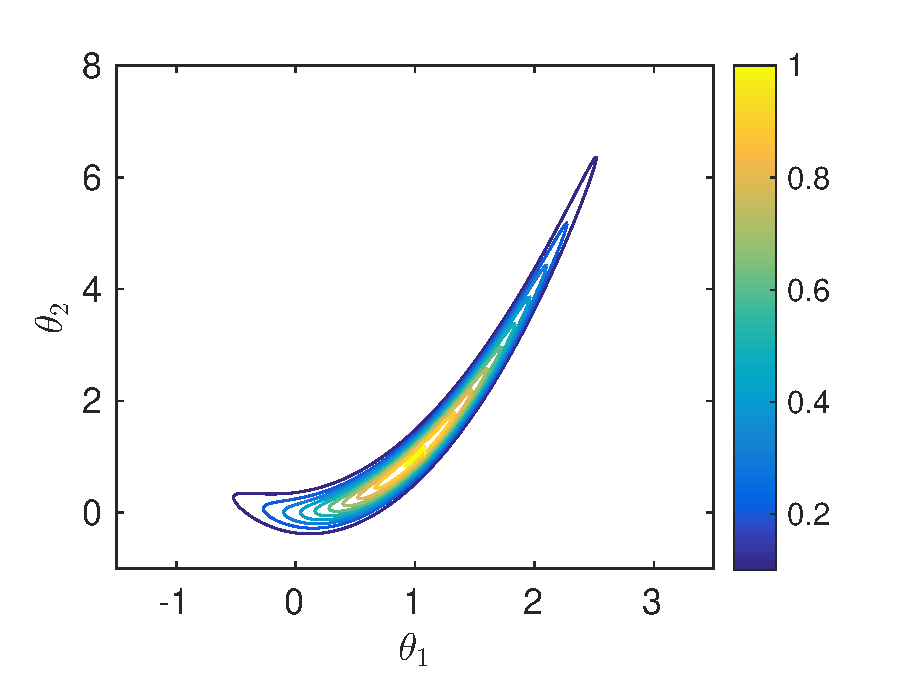
\includegraphics[width=0.31\textwidth]{images/TPAIS/R2_posterior}}
\caption{Visualisation of the Rosenbrock density as given in Equation~\eqref{eqn:R2_repeat}.}
\label{fig:R2_posterior}
\end{figure}
This problem is challenging to sample from since it has a highly peaked and curved ridge, and is often used
as a test problem in optimisation and MCMC communities.

\subsection{Implementation details}

Before looking at the performance of the MCMC algorithms, we demonstrate some properties of the transport maps we will be using in our MCMC algorithms. We draw 1 million samples from the density in \eqref{eqn:R2_repeat}, and use this sample in the framework of Section~\ref{sec:map} to build a transport map. We use this map to push forward the original sample onto the reference space, where we will be able to see how well the map has performed at converting the original sample to a standard Gaussian. We then pull the sample back on to target space using the inverse map to check that our map is invertible and well behaved.

For this example, we use an index set of total order 3 with monomial
basis functions. It is important that total order is an odd number,
since otherwise the map will not be surjective. This results in a map of the form
\[
	T(\theta_1, \theta_2) = \begin{bmatrix} T_1(\theta_1) \\ T_2(\theta_1, \theta_2) \end{bmatrix},
\]
where
\begin{align*}
		T_1(\theta_1) &= \gamma_{1,1} + \gamma_{1,2}\theta_1 + \gamma_{1,3}\theta_1^2 + \gamma_{1,4}\theta_1^3, \\
		T_2(\theta_1, \theta_2) &= \gamma_{2,1} + \gamma_{2,2}\theta_1 + \gamma_{2,3}\theta_1^2 + \gamma_{2,4}\theta_1^3
					+ \gamma_{2,5}\theta_2 + \gamma_{2,6}\theta_1\theta_2 \\
				 & \qquad \quad + \gamma_{2,7}\theta_1^2\theta_2 + \gamma_{2,8}\theta_2^2 + \gamma_{2,9}\theta_1\theta_2^2 +
					 \gamma_{2,10}\theta_2^3.
\end{align*}
Clearly even with only basis functions of total order 3, we have a large number of unknowns in our optimisation problem, $\bar{\gamma} \in \mathbb{R}^{14}$. If we were to increase the dimension of $\theta$ further we would need to reduce the number of terms we include in the expansion by, for example, removing all the ``cross'' terms. This reduces the quality of our map but since we only require an approximate map we can afford to reduce the accuracy.

\begin{figure}[htpb]
\centering
\subfigure[Original sample $\theta$ from MH-RW algorithm.]{\includegraphics[width=0.31\textwidth]{"images/TPAIS/R2_transport_orig"}}\quad
\subfigure[Push forward of $\theta$ onto reference space.]{\includegraphics[width=0.31\textwidth]{"images/TPAIS/R2_transport_ref"}}\quad
\subfigure[Pull back of reference sample onto target space.]{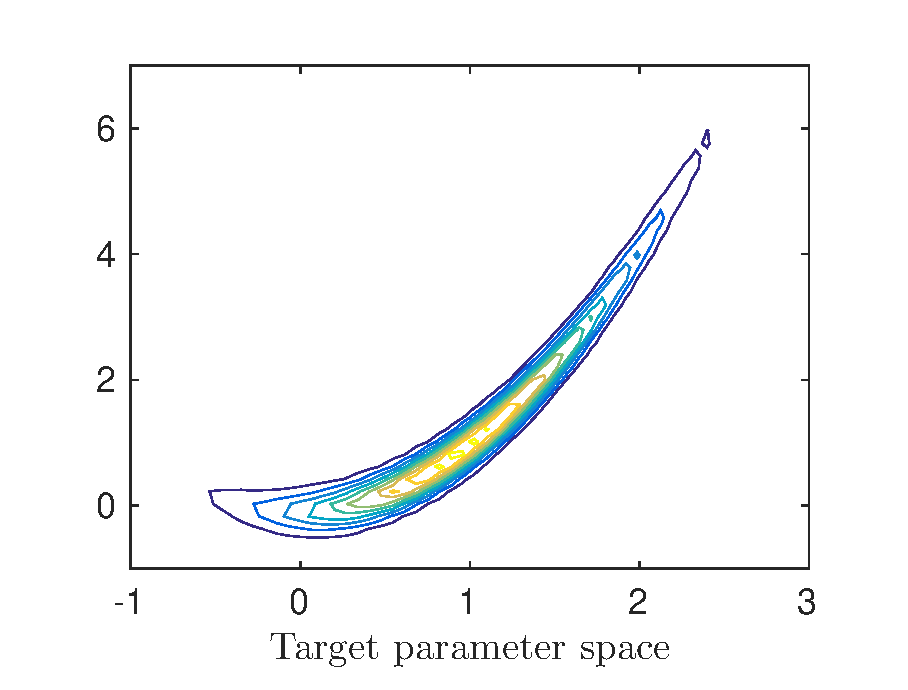
\includegraphics[width=0.31\textwidth]{images/TPAIS/R2_transport_pullback}}
\caption{The effect of the approximate transport map $\tilde{T}$ on a
  sample from the Rosenbrock target density as described in Equation~\eqref{eqn:R2_repeat}.}
\label{fig:R2_transport}
\end{figure}

Figure~\ref{fig:R2_transport} shows the output of the approximate
transport map. Even though we have truncated the infinite expansion in
the monomial basis down to 4 and 10 terms in respective dimensions,
the push forward of the sample is still a unimodal distribution
centred at the origin with standard deviation 1. As you move out into
the tails of the reference density more non-Gaussian features are
clearly visible. However, overall, the push forward of the target
density does not look a challenging one to sample from, with even
relatively simple MCMC methods such as MH-RW. The pullback from
reference space, in Figure~\ref{fig:R2_transport}, is an exact match
of the original sample since we have not perturbed the sample in
reference space. This inversion is well defined in the sampling
region, although not necessarily outside\cite{parno2014transport}.

\subsection[Numerical results]{Numerical results for convergence of
  transport map based algorithms on the Rosenbrock density}

We first find the optimal scaling parameters for the individual
algorithms. This is done, as in \cite{cotter2015parallel}, by optimising for the effective sample size in
the PAIS algorithm, and by tuning the relative $L^2$ error in the MH
algorithm. There is currently no
guidance on the best way of tuning the MH algorithm with transport map
proposals although one might expect results similar to the standard MH
results, especially if adaptation of the map is stopped after a given
point. As in the PAIS algorithm, optimising for the effective sample size might be the best option.

\begin{table}[!ht]
\centering
\begin{tabular}{lrrr}
\toprule
	Statistic \quad / \quad Algorithm & Transport M-H &
                                                            Alg. \ref{alg:TransportPAIS1} & Alg. \ref{alg:TransportPAIS2}  \\ \cmidrule(lr){1-4}
	$\delta_{L^2}$				 & 1.0e-0 & 1.1e-1 & 3.5e-1 \\
	$\delta_{\text{ESS}}$				 & - & 1.0e-1 & 5.2e-1 \\ \cmidrule(lr){1-4}
	Acc. rate							 & 0.23 & - & - \\
	ESS ratio							 & - & 0.62 & 0.71 \\
\bottomrule
\end{tabular}
\caption{Optimal scaling parameters for the transport map based
  algorithms applied to $R_1$, optimising for the $L^2$ error and
  the effective sample size (ESS) for PAIS algorithms, and for average
  acceptance rate for MH algorithms.}
\label{tab:R2_opt_scaling}
\end{table}

The optimal scaling parameters are given in
Table~\ref{tab:R2_opt_scaling}. Here we see that the effective sample
size is much lower than we see in the one-dimensional examples with
the PAIS algorithms. However, in the Rosenbrock density
\eqref{eqn:R2_repeat} we are dealing with a much more complicated
correlation structure, as well as a very slowly decaying tail in
$\theta_2$. From our experiments, we have observed that the standard PAIS-RW required an ensemble size of $M=500$ to overcome the problems in this density, however the transport map transforms the tails to be more like those of a Gaussian which can be approximated well by a smaller ensemble size of $M=150$.

\begin{figure}[!ht]
\centering
\subfigure[Comparison of the two Transport PAIS options.]{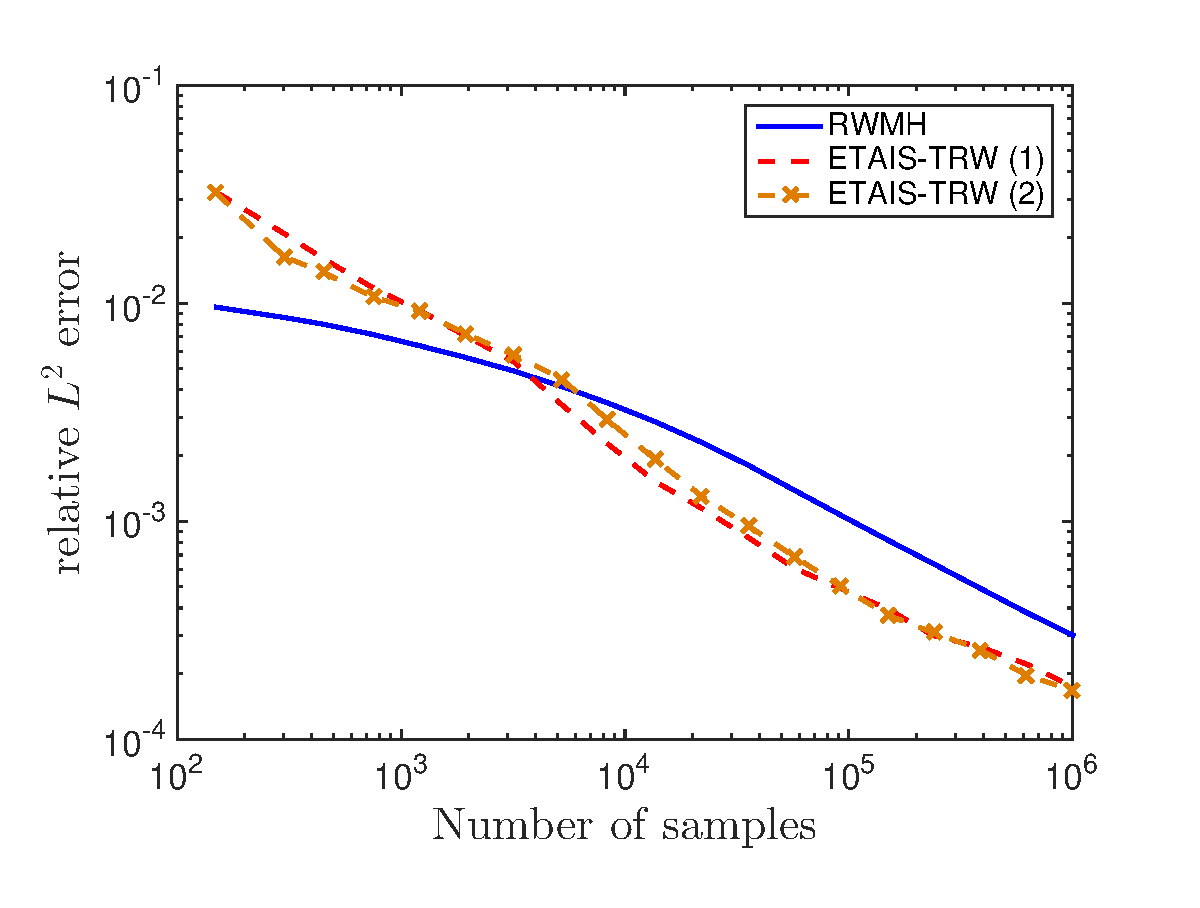
\includegraphics[width=0.45\textwidth]{images/TPAIS/R1_L2}}
\subfigure[Comparison of Transport PAIS option (2) with the standard algorithms.]{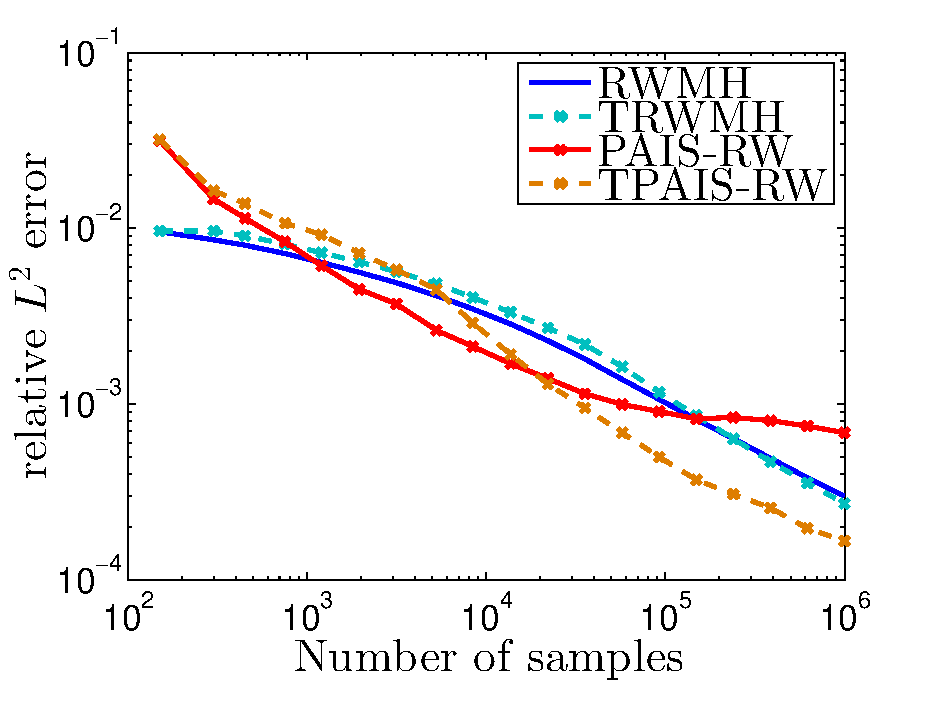
\includegraphics[width=0.45\textwidth]{images/TPAIS/R1_L2_all}}
\caption{Convergence of algorithms; Transport M-H,
  algorithm \ref{alg:TransportPAIS1}, algorithm \ref{alg:TransportPAIS2} for
  density \eqref{eqn:R2_repeat}. Ensemble size $M=150$, resampling performed using the AMR algorithm.}
\label{fig:R2_l2_convergence}
\end{figure}

The convergence of the three algorithms is displayed in Figure~\ref{fig:R2_l2_convergence}. Figure (a) shows that the two variations of the transport based PAIS algorithms converge with similar rates. The second version, which performs the resampling stage in reference space rather than target space, has a slightly higher ESS, and is more stable than option (1). This version also has a property that we can exploit in Section~\ref{sec:TPAIS_higher_dim}.


%\section{Transport map-accelerated Parallel Adaptive Importance
  %Sampling (TPAIS)}\label{sec:TPAIS}

\section{Multiscale Methods for Stochastic Chemical Reaction
  Networks}\label{sec:multi}
In this Section, we discuss some recent advances in multiscale methods
for stochastic reaction networks. Inverse problems arising in this
area often lead to highly correlated and complex posterior
distributions, which traditional MCMC methods can struggle to sample
from. We will then go on to solve some inverse problems related to
this in Section \ref{sec:num}, using the transport map versions of the
PAIS algorithm, as described in Section \ref{sec:TPAIS}.

We consider chemical reaction networks of $N_s$ chemical species $\{S_j\}_{j=1}^{N_s}$,
with population numbers given by $X(t) = [X_1(t), X_2(t), \ldots, X_{N_s}(t)]^\top \in
\mathbb{N}_0^{N_s}$ reacting in a small reactor, through $N_r$ different reaction
channels. When population numbers of one or more of the chemical
species in the reactor is small, as is the case with chemical
reactions occurring within living cells, the sporadic and discrete way
in which reactions occur can not be well modelled by deterministic
continuous models, such as ODEs. In such a situation, we may wish to
model the dynamics through a discrete stochastic model, such as a
continuous time Markov chain.

For each reaction $R_j$, for $j = 1,2,\ldots N_r$, there is a
propensity or hazard function $\alpha_j(X(t)$ which indicates how
likely that reaction is to fire, defined by
\[\alpha_j(X(t)) = \lim_{dt \to 0} \mathbb{P}(\text{Reaction $R_j$ in
    the time interval  } \quad s \in [t, t+ dt] ).\] If a system
satsifies what is called \emph{mass action kinetics}, then the form of
the function $\alpha_j$ is determined, up to a rate constant, by the
reactants involved in that reaction:
\begin{equation}\label{eq:MAK}
\alpha_j(X) = k_j \prod_{m=1}^{N_s} \prod_{n=0}^{\nu_{j,m} -1} (X_m - n),
\end{equation}
where $\nu_{j,m}$ is the $m$th component of the stoichiometric vector
$\nu_j$, $X_m$ is the $m$th component of the state vector $X$, and the
$k_j$ are rate constants.

Following each reaction $R_j$ there is an instantaneous change in the
current state, as the reactants of the reaction are consumed, and the
products produced. This is modelled by a change in the state vector
$X(t) = X(t) + \nu_j$ where $\nu_j$ is that stochiometric vector for
reaction $R_j$.

The model can be represented as the following expression involving
$N_r$ different unit rate Poisson
processes\cite{anderson2011continuous} $Y_j$, given by:
\begin{equation}\label{eq:RTC}
X(t) = X(0) + \sum_{j=1}^{N_r} \nu_j \int_0^t \alpha_j(X(s)) ds.
\end{equation}

The master equation for this model is only solvable in certain
situations, for example monomolecular networks\cite{jahnke2007solving}, or for
steady-state solutions certain deficiency
zero networks\cite{anderson2010product,anderson2016product}. Trajectories for this system can be
sampled exactly, for instance using the Gillespie SSA\cite{gillespie1977exact}, or
its variants\cite{gillespie2007stochastic,gibson1998efficient,cao2004efficient,anderson2007modified}. However, if the system is stiff, i.e. there
are some reactions which are firing many times on a timescale for
which others are unlikely to fire at all, then trajectories can become
prohibitively expensive to simulate, since these methods simulate
every single reaction event with the same cost. In such a system, one
might employ multiscale methods in order to approximate trajectories
at a lower cost than the exact algorithms.

One common approach is to induce the quasi-steady-state approximation
QSSA. This approximation makes the assumption that fast reactions
enter quasi-equillibrium on a timescale which is negligible with
respect to the timescale on which the slow dynamics in the system are
evolving. This amounts to taking the assymptotic limit that the
propensities of the ``slow'' reaction channels are equal to zero. This
allows us to sample approximate trajectories of the slow reactions
without the need to compute many fast reaction events.

This approach can work well when there is a large timescale gap
between the fast and slow reactions in a system, but where the
timescale gap is less pronounced, it can lead to significant
errors\cite{cotter2016error}. Another approach is the
constrained multiscale method (CMA)\cite{cotter2011constrained,cotter2016constrained}, based in part on the
equation-free approach to multiscale computations\cite{kevrekidis2003equation,erban2006gene}. This approach also assumes quasi-equillibrium in the
system, but takes into account the effect that the slow reactions can
have on the invariant distribution of the fast variables in the
system. For a more detailed description of this method, please refer
to the literature\cite{cotter2016constrained}.

Multiscale methods are not only of use when forward evaluations of the
dynamics are costly, but can also be of use where we attempt to solve
an inverse problem where the fast variables are unobservable. One
approach in this situation would be to integrate over all possible
trajectories of the fast variables, but this would almost always be
prohibitively expensive. Another approach would be to use an
appropriate multiscale approximation, so that the effective dynamics
of the slow variables can be approximate without the need to consider
the rapid fluctuations of the fast variables in the system.

\subsection{Likelihoods arising from stochastic reaction networks}
Suppose that we are able to exactly observe the number of molecules of
each chemical species in a system which satisfies mass action
kinetics, and which can be well approximated by
\eqref{eq:RTC}. Suppose that we wish to be able to infer the value of
the rate constants of each reaction from these observations. Even with no observational noise, since the dynamics
of the system are stochastic, this still leads to a Bayesian inverse
problem where we can only infer a joint probability distributions on the
reaction parameters.

Suppose that we are in state $X(t) = X_0$. There are two independent
univariate random variables which decide when and what the next
reaction in the system is. There is the $j$th waiting time $\tau_j$ to the
next reaction, which is given by an exponential random variable
\[\tau_j \sim \exp \left ( \frac{1}{\alpha_0(X(t))} \right ),\]
where $\alpha_0(X(t)) =\sum_{i}^{N_r} \alpha_i(X(t))$ is the total
propensity in the system. The second is a multinomial random variable $r_j$
which dictates which reaction has occurred during the $j$th reaction,
which takes the value
$r \in \{1,2,\ldots,N_r\}$ with probability
\[\mathbb{P}(r = i) = \frac{\alpha_i(X(t))}{\alpha_0(X(t))}.\]
As such, in order to compute the likelihood of a particular trajectory
given a possible realisation of the reaction parameters, it is
sufficient to have access to the total time spent in each state, and
the frequency of each reaction which led to leaving each state.

From this formulation, we see that the random variables $(\tau_j, r_j)$ only depend on the states $\mathbf{X}(t_{j-1})$ and so are Markovian. This conditional independence means that we can group events together by what state the system was in when the event happened. We define two new random variables which depend on a state $\mathbf{Y} \in \mathcal{S}$, first the total time spent in state $\mathbf{Y}$,
\[
	T(\mathbf{Y}) = \sum\limits_{j=1}^M \tau_j\; \text{I}(\mathbf{X}(t_{j-1}) = \mathbf{Y}).
\]
This random variable, $T(\mathbf{Y})$, is a sum of exponentially
distributed random variable, each with the rate $\alpha_0(\mathbf{Y};\mathbf{k})$, and hence follows the Gamma distribution,
\begin{equation}\label{eqn:chem_time_dist}
	T(\mathbf{Y}) \sim \text{Gamma}\left(\alpha=K(\mathbf{Y}),~\beta = \alpha_0(\mathbf{Y}; \mathbf{k})\right),
\end{equation}
where $K(\mathbf{Y}) = \sum\limits_{j=1}^M \text{I}(\mathbf{X}(t_{j-1}) = \mathbf{Y})$.

Similarly, we can define the reactions which occurred when the system was in state $\mathbf{Y}$ as $\mathbf{r}(\mathbf{Y}) = [r_1(\mathbf{Y}), \ldots, r_{N_r}(\mathbf{Y})]^\top$ where
\[
	r_i(\mathbf{Y}) = \sum\limits_{j=1}^M \text{I}(r_j = i \textbf{ and }\mathbf{X}(t_{j-1}) = \mathbf{Y}).
\]
Here all the random variables $r_j$ follow the same multinomial distribution, and so
\begin{equation}\label{eqn:chem_react_dist}
	\mathbf{r}(\mathbf{Y}) \sim \text{Multinomial}(K(\mathbf{Y}),~\mathbf{p}(\mathbf{Y})). 
\end{equation}
The random variables defined in Equations~\eqref{eqn:chem_time_dist} and \eqref{eqn:chem_react_dist} are sufficient statistics for the posterior distribution $\pi(\mathbf{k}|D)$. With these definitions we define two new structures
\[
	\mathbf{T} = [T(\mathbf{Y}_1), \dots, T(\mathbf{Y}_K)]^\top, \quad \text{and} \quad \mathbf{R} = [\mathbf{r}(\mathbf{Y}_1), \dots, \mathbf{r}(\mathbf{Y}_K)]^\top,
\]
where $K = |\mathcal{S}|$, the number of states in $\mathcal{S}$, and each state $\mathbf{Y}_i \in \mathcal{S}$ has been enumerated. We use these structures to define shorter notation,
\[
	\mathbf{T}_i = T(\mathbf{Y}_i), \quad \mathbf{R}_{ij} = r_j(\mathbf{Y}_i), \quad \text{and} \quad \mathbf{K}_i = K(\mathbf{Y}_i).
\]

To construct the posterior distribution for the reaction rates, $\mathbf{k}$, in the chemical system, we formulate the likelihood using the sufficient statistics derived in the previous section. Due to the non-negativity of these reaction rates, we assign a Gamma prior distribution to each rate. Given the distributions in Equations~\eqref{eqn:chem_time_dist} and~\eqref{eqn:chem_react_dist} for our data, the likelihood of observing the data $\mathbf{R}$ and $\mathbf{T}$ is
\[
	\ell(\mathbf{R}, \mathbf{T}|\mathbf{k}) \propto \prod\limits_{i=1}^K \text{Multi}(\mathbf{r}(\mathbf{Y}_i); \mathbf{K}_i, \mathbf{p}(\mathbf{Y}_i))\text{Gamma}(\mathbf{T}_i; \mathbf{K}_i, \alpha_0(\mathbf{Y}_i)),
\]
where again $\mathbf{Y}_i \in \mathcal{S}$ and the propensities
$\alpha_i$ and probabilities $p_i$ depend on the reaction rates
$\mathbf{k} = [k_1, k_2, \ldots k_{N_r}]^\top$ through the concept of
mass action kinetics given in \eqref{eq:MAK}.

Our choice of Gamma prior distributions with hyper-parameters $(a_i, b_i)$ results in the posterior distribution of the form
\begin{align}
	\pi(\mathbf{k}|\mathbf{R}, \mathbf{T}) &\propto \ell(\mathbf{R}, \mathbf{T}|\mathbf{k})
	\prod_{i=1}^{N_r} \! \text{Gamma}(k_i; a_i, b_i) \notag \\
		&\propto \exp\Bigg\{\sum\limits_{i=1}^K \Bigg[
				\mathbf{K}_i\log \alpha_0(\mathbf{Y}_i; \mathbf{k}) - \mathbf{T}_i\alpha_0(\mathbf{Y}_i; \mathbf{k}) %\notag \\
%		& \qquad\qquad\qquad
				+\sum_{j=1}^{N_r} \mathbf{R}_{ij}\log\mathbf{p}_j(\mathbf{Y}_i; \mathbf{k})
			\Bigg]  \notag\\
		&	\qquad\qquad\qquad{} + \sum_{i=1}^{N_r} ((a_i-1)\log k_i - b_ik_i)\Bigg\}. \label{eqn:chem_posterior}
\end{align}

\subsection{Approximation of likelihoods in multiscale chemical
  networks}
Suppose now that we are only observing the slower variables in a
multiscale chemical system of this type. Suppose that $n_r < N_r$ is the number of slow
reactions in the system, and the slow reactions are given by $\{R_{s_1},
R_{s_2}, \ldots R_{s_{n_r}} \} \subset \{R_1, R_2, \ldots , R_{N_r}
\}$. The propensities of the slow
reactions $\alpha_{s_i}$ may depend on the value of the fast variables which is
unknown. However, the invariant distribution of the fast variables
conditioned on the slow variables in the system can be approximated
using a multiscale method, such as the QSSA or the CMA, as described
briefly in Section \ref{sec:multi}. Once the approximations have been
made, we arrive at approximate \emph{effective} propensities $\bar{\alpha}_{s_i}$, which
have been averaged over the computed invariant distributions of the
fast variables. Then the approximate effective dynamics on the slow variable $S(t)$ are given by 
\begin{equation}\label{eq:RTCS}
S(t) = S(0) + \sum_{j=1}^{n_r} \nu_{s_j} \int_0^t \bar{\alpha}_{s_j}(S(s)) ds.
\end{equation}

In turn, the approximate posterior distribution on the reaction
parameters $\mathbf{k}$ is then given by
\begin{align}
	\pi(\mathbf{k}|\mathbf{R}, \mathbf{T}) &\propto \ell(\mathbf{R}, \mathbf{T}|\mathbf{k})
	\prod_{i=1}^{n_r} \! \text{Gamma}(k_i; a_i, b_i) \notag \\
		&\propto \exp\Bigg\{\sum\limits_{i=1}^K \Bigg[
				\mathbf{K}_i\log
                  \bar{\alpha}_0(\mathbf{Y}_i; \mathbf{k}) -
                  \mathbf{T}_i \bar{\alpha}_0(\mathbf{Y}_i; \mathbf{k}) %\notag \\
%		& \qquad\qquad\qquad
				+\sum_{j=1}^{n_r} \mathbf{R}_{ij}\log \bar{\mathbf{p}}_j(\mathbf{Y}_i; \mathbf{k})
			\Bigg]  \notag\\
		&	\qquad\qquad\qquad{} + \sum_{i=1}^{n_r} ((a_i-1)\log k_i - b_ik_i)\Bigg\}, \label{eq:Apos}
\end{align}
where $\bar{\alpha}_0(\mathbf{Y}_i; \mathbf{k}) = \sum_{j=1}^{n_r}
\bar{\alpha}_j(\mathbf{Y}_i; \mathbf{k})$ is the total of the
effective propensities, $n_r$ is the number of slow reactions,
$\bar{\mathbf{p}}(\mathbf{Y}_i; \mathbf{k})$ is the multiscale
approximation of the expected proportion of each slow reaction at
state $\mathbf{Y}_i$ and with reaction rates $\mathbf{k}$ and the
data is limited only to changes in the slow variable due to the
occurrence of slow reactions.
\section{Numerical Examples}\label{sec:num}
In this section we look at two examples of chemical systems to
demonstrate the effectiveness of the Bayesian approach we have
proposed, along with the transport PAIS algorithms for sampling the
challenging posterior distribution on the reaction parameters that
arise. 

% The first example will only contain at most mono-molecular reactions,
% i.e. reactions which convert one species into another species at a
% particular rate. As shown in~\cite{jahnke2007solving} these systems
% have a Poisson invariant distributions on the populations, given by
% \begin{equation}\label{eqn:mono_stat_dist}
% 	\mathbb{P}(X_1=x_1, \ldots, X_n=x_n) = \left(\prod_{i=1}^n \! \frac{\bar{c}_i^{x_i}}{x_i!}\right)\exp\left(-\sum_i^n \! \bar{c}_i\right),
% \end{equation}
% where $x_i \in \mathbb{N}$ and $\bar{c}_i$ are the complex balances or the concentration of chemical $X_i$ according to the solution of a steady state approximation of the system. We make use of this distribution to formulate posteriors for the chemical reaction rates using the constrained multiscale approach, as in~\cite{cotter2016constrained}.

%%%%%

\subsection{A Multiscale Chemical System}\label{sec:chem_multiscale}

First we consider a simple multiscale example involving two chemical
species $S_1$ and $S_2$ involved in only zeroth and first order reactions:
\begin{equation}\label{eqn:full_system}
	\emptyset \xrightarrow{k_1} S_1 \xleftrightarrows[k_3]{k_2} S_2 \xrightarrow{k_4} \emptyset.
\end{equation}
Each arrow represents a reaction from a reactant to a product, with
some rate constant $k_i$, and where mass action kinetics is
assumed. The parameters $k_i$ are non-negative, and $\mathbf{k} =
[k_1,\dots,k_4]^\top \in \mathbb{R}_+^4 = \mathcal{X}$. We denote the
population count of
species $S_i$ by $X_i \in \mathbb{N}_0$. 
We consider this system with the following parameters:
\begin{equation}\label{eq:params1}
k_1 = 100, \qquad k_2 = k_3 = 10, \qquad k_4 = 1,
\end{equation} 

 In this 
parameter regime the reactions $R_2\colon S_1\rightarrow S_2$ and $R_3\colon S_2\rightarrow S_1$ occur
more frequently than the other reactions. Notice that both
chemical species are involved in fast reactions. However, the quantity
$S = X_1 + X_2$, is conserved by both of the fast reactions,
and as such, this is the slowly changing quantity in this system.

We observe this system over the time period $t \in [0,500]$ with
initial condition ******, but we assume that we are only able to observe
the slow variable $S(t)$. 
The effective dynamics of $S$ can be approximated by a system of only
two reactions:
\begin{equation}\label{eqn:QSSA_system}
	\emptyset \xrightarrow{\alpha_1(S)} S \xrightarrow{\bar{\alpha}_4(S)} \emptyset,
\end{equation}
where here the propensities are shown as opposed to the rates.

The effective propensity $\bar{\alpha}_4(S)$ can be  approximated through
application of a multiscale approximation, as detailed in Section
\ref{sec:multi}, and in more detail in \cite{cotter2016constrained}. These effective
propensities can often be computed without the need for expensive
simulations, in particular when the fast subsystem is deficiency zero,
which is often the case\cite{anderson2010product,anderson2016product}. For this very
simple example, the dependance of these effective
propensities on the original rate parameters can be explicitly
understood. Under the QEA,
the effective rate of degradation of the slow variable $S$ is given by
\[
	\bar{\alpha}_4^{\text{QEA}}(s) = \frac{k_2k_4s}{k_2+k_3}.
\]
Similarly, the analysis of the constrained system as discussed in~\cite{cotter2016constrained} yields the effective propensity
\begin{equation}\label{eqn:chem_CMA_rate}
	\bar{\alpha}_4^{\text{CMA}}(s) = \mathbb{E}_{\text{CMA}}\left[k_4X_2|S=s\right] = \frac{k_2k_4s}{k_2+k_3+k_4}.
\end{equation}

Our observations are uninformative about the reaction rates $k_2,
k_3$, and $k_4$, as for each multiscale approximation there
is a manifold $\mathcal{M} \subset \mathcal{X}$ along which the effective propensity
$\hat{\alpha}_4$ is invariant, leading to a highly ill-posed inverse
problem. This type of problem is notoriously difficult to
sample from using standard MH algorithms, as the algorithms quickly
gravitate towards the manifold $\mathcal{M}$ but then
exploration around $\mathcal{M}$ is slow.

We aim to recover three different posterior distributions. In the
first, which is of the form \eqref{eqn:chem_posterior}, we assume that we can fully and exactly observe the whole state
vector for the whole of the observation time window $t \in [0,T]$. In
the second and
third, the same data are used, but restricted to observations of the slow
variable $S = X_1 + X_2$. In these last two examples, we approximate the
posterior using \eqref{eq:Apos} with QEA and CMA approximations of the
effective dynamics respectively.

In all three cases, we find the posterior distribution for $\mathbf{k} \in \mathcal{X}$. These four parameters are assigned Gamma prior distributions,
\[
	k_i \sim \text{Gamma}(\cdot; \alpha_i, \beta_i), \quad \text{for} \quad i = 1, \dots, 4.
\]
The hyper-parameters corresponding to each of these prior distributions are given in Table~\ref{tab:multiscale_priors}. These priors are the same for each of the three posterior distributions.

\begin{table}
\centering
\begin{tabular}{|l|R{2em}R{2em}R{2em}R{2em}|}
	\hline
	Parameter$\backslash$Dimension $i$ & 1 & 2 & 3 & 4 \\ \hline
	$\alpha_i$ & 150 & 5 & 5 & 3 \\
	$\beta_i$ & $\frac{15}{9}$ & $\frac{5}{12}$ & $\frac{5}{12}$ & $1$ \\ \hline 
\end{tabular}
\caption{Hyper-parameters in the prior distributions for the multiscale problem described in Section~\ref{sec:chem_multiscale}.}
\label{tab:multiscale_priors}
\end{table}

\begin{figure}[htb]
\centering
\includegraphics[width=0.9\textwidth]{"images/Applications/CMA_posterior"}
\caption{CMA approximation \eqref{eq:Apos} of the posterior arising from observations of
  the slow variable $S = X_1 + X_2$ for system
  \eqref{eqn:full_system}  with true rates given by \eqref{eq:params1}.}
\label{fig:chem_CMA_posterior}
\end{figure}

Figure~\ref{fig:chem_CMA_posterior} shows how this posterior looks
when we use the CMA to model the effective degradation propensity $\bar{\alpha}_4$.

We consider several different algorithms for sampling from these
distributions. First we implement both the PAIS and MH algorithms with
a Gaussian proposal distribution. In the case of the PAIS algorithm,
this is a Gaussian mixture proposal distribution, and in the MH
algorithm this is equivalent to a vanilla random walk. The proposal distribution uses a covariance matrix which has been constructed using the sample covariance of a sample produced using a standard MH-RW algorithm. We also compare the PAIS and MH algorithms when using a transport map proposal distribution. This proposal method was discussed in detail in Chapter~\ref{sec:TPAIS}.

\begin{figure}
	\centering
	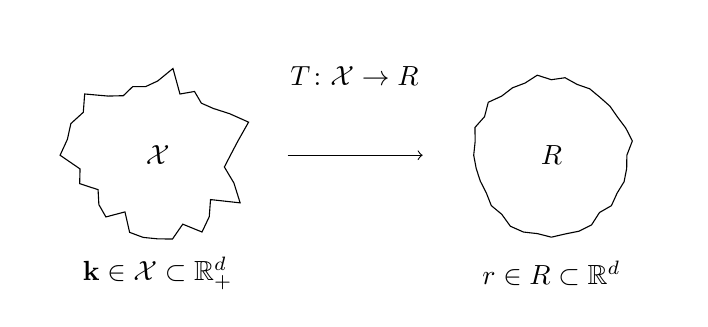
\begin{tikzpicture}
		\pgfmathsetseed{1}

		\node[inner sep=1.5cm,outer sep=0] (A) at (0,0) {$\mathcal{X}$};
		\node[inner sep=1.5cm,outer sep=0] (B) at (5,0) {$R$};

		\draw (A) \irregularcircle{1cm}{2.5mm};
		\draw (B) \irregularcircle{1cm}{0.5mm};

		\draw [->] (A) -- (B);

		\node at (2.5,1) {$T\colon\mathcal{X}\rightarrow R$};

		\node at (0,-1.5) {$\mathbf{k}\in\mathcal{X}\subset\mathbb{R}_+^d$};
		\node at (5,-1.5) {$r\in R\subset\mathbb{R}^d$};
	\end{tikzpicture}

	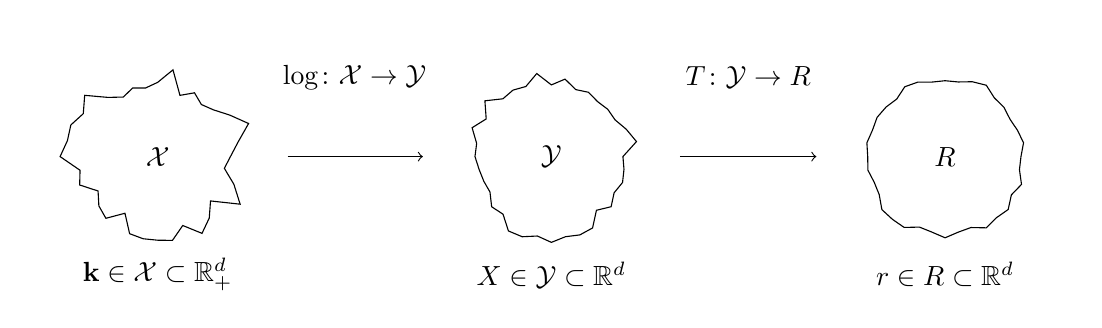
\begin{tikzpicture}
		\pgfmathsetseed{1}

		\node[inner sep=1.5cm,outer sep=0] (A) at (0,0) {$\mathcal{X}$};
		\node[inner sep=1.5cm,outer sep=0] (B) at (5,0) {$\mathcal{Y}$};
		\node[inner sep=1.5cm,outer sep=0] (C) at (10,0) {$R$};

		\draw (A) \irregularcircle{1cm}{2.5mm};
		\draw (B) \irregularcircle{1cm}{1.1mm};
		\draw (C) \irregularcircle{1cm}{0.5mm};

		\draw [->] (A) -- (B);
		\draw [->] (B) -- (C);

		\node at (2.5,1) {$\log\colon\mathcal{X}\rightarrow\mathcal{Y}$};
		\node at (7.5,1) {$T\colon\mathcal{Y}\rightarrow R$};

		\node at (0,-1.5) {$\mathbf{k}\in\mathcal{X}\subset\mathbb{R}_+^d$};
		\node at (5,-1.5) {$X\in\mathcal{Y}\subset\mathbb{R}^d$};
		\node at (10,-1.5) {$r\in R \subset\mathbb{R}^d$};
	\end{tikzpicture}
	\caption{Couplings between parameter space and reference
          when using the transport map with (bottom) and without (top)
        a log preconditioner.}
	\label{fig:chem_coupling}
\end{figure}

Figure~\ref{fig:chem_coupling} (top) shows how we define a bijective map,
$\hat{T}$, between parameter space $\mathcal{X}$ and a reference space
$R$. When using the transport map proposal distribution, we prefix the proposal method with a T, e.g. MH-RW  and MH-TRW, as well as PAIS-RW and PAIS-TRW. In practice we cannot ensure that the approximate map $\tilde{T}$
is uniquely invertible over the whole of $R$ and so $\tilde{T}$ is not
truly bijective. This leads to problems for our strictly positive
state space, $\mathcal{X} \subset \mathbb{R}_+^d$, since proposals in
$R$ do not necessarily map back onto $\mathcal{X}$.

Therefore we also consider how these algorithms perform when the transport map
is preconditioned by the logarithmic function applied to the parameters. We choose to use this log
preconditioner since it converts our strictly positive parameter
space, $\mathcal{X}$, into an intermediate space $\mathcal{Y} \subset
\mathbb{R}^d$. This allows us to define $T$ between two subsets of
$\mathbb{R}^d$, which means that all proposals made on the reference
space are mapped to valid
proposals on the true parameter space. It also reduces the work required of the map, which since
we use only a finite dimensional approximation, can improve
performance and stability. As before, the proposal distributions are labelled with a T for transport map and when using the intermediate space we prepend `log' to the proposal method, e.g. MH-logRW and MH-logTRW, with, PAIS-logRW and PAIS-logTRW.

Figure~\ref{fig:chem_coupling} (bottom) displays the composition of maps
when we include this $\log$ preconditioner leading to an intermediate space $\mathcal{Y}$. The inclusion of this additional map means that we must again alter our importance weight definition to reflect the pullback from $R$ through $\mathcal{Y}$. The weight is now
\[
	w_i(\theta) = \frac{\pi(\theta|\mathbf{R},\mathbf{T})}{\chi(\tilde{T}\circ\log(\theta)|\tilde{T}\circ\log(\theta^{(i-1)}))|J_{\tilde{T}\circ\log}(\theta)|},
\]
where $\theta$ is a proposed new state, $\theta^{(i-1)}$ is the ensemble of states from the previous iteration, and $J_{\tilde{T}\circ\log}(\theta)$ is the Jacobian of the composition of the two maps. This Jacobian is straightforward to calculate,
\[
	|J_{\tilde{T}\circ\log}(\theta')| = |J_{\tilde{T}}(\log(\theta'))||J_{\log}(\theta')|,
\]
where the first determinant is computed as in
\eqref{eqn:separable_jacobian}, and the second is given by
\[
	|J_{\log}(\theta')| = \prod\limits_{i=1}^d \frac{1}{\theta'_i}.
\]

% choices made in transport map
For this problem, we continue to use monomials in each dimension in our transport map construction. We use polynomials of total order $p=3$ as the basis functions, i.e.
\[
	T_i(\theta) = \sum_{\mathbf{j}\in\mathcal{J}^{\text{TO}}_i(p)} \gamma_{i,\mathbf{j}}\psi_{\mathbf{j}}(\theta) \quad \text{where} \quad \psi_\mathbf{j}(\theta) = \prod\limits_{k=1}^i \theta_k^{j_k},
\]
and
\[
	\mathcal{J}^{\text{TO}}_i(p) = \{\mathbf{j} \in \mathbb{N}^d_0\ |\ \|\mathbf{j}\|_1 \leq p, \ \text{and}\ j_k = 0\ \forall k > i\}.
\]

% choice of resampler?
We will use the AMR\cite{russ2017parallel} resampler with an ensemble size of
$M=500$. This increase in ensemble size in comparison with previous
example in Section \ref{sec:conv} is to allow for the increase in parameter dimension.

% analysis method
To measure the convergence of the sampling methods in this section, we
will compare the convergence of the mean of each parameter. We
approximate $\mathbb{E}(\mathbf{k})$ using 2.4 billion samples from
the MH-RW algorithm. We do this for each of the eight algorithms we
have so far discussed. Convergence is shown only for the CMA
approximation of the posterior \eqref{eq:Apos} with effective rate for
the degradation of $S$ given by \eqref{eqn:chem_CMA_rate}, but we
expect very similar results for the other posterior distributions discussed.

\begin{table}[!h]
\centering
\begin{tabular}{rrrrrr}
\toprule
	\multicolumn{1}{l}{Algorithm} & \multicolumn{3}{c}{MH} & \multicolumn{2}{c}{PAIS} \\ \cmidrule(lr){2-4} \cmidrule(lr){5-6}
	& & $\delta$ & & $\delta$ & ESS \\ \midrule
	RW & & 5.5e-3 & & 1.0e-0 & 9.0e-3 \\
	TRW & & 1.2e-0 & & 4.0e-1 & 1.2e-3 \\
	logRW & & 1.7e-1 & & 1.2e-0 & 6.0e-2 \\
	logTRW & & 2.7e-2 & & 1.5e-1 & 3.5e-1 \\
\bottomrule
\end{tabular}
\caption{Optimal scaling parameters for the MH and PAIS algorithms applied to the constrained multiscale problem in Section~\ref{sec:chem_multiscale}. MH parameters optimised by acceptance rate, and PAIS parameters optimised using effective sample size.}
\label{tab:chem_multiscale_scaling}
\end{table}

The optimal scaling parameters for the proposal distributions are
given in Table~\ref{tab:chem_multiscale_scaling}. These are
precomputed by running the algorithms for different parameter
values. MH-RW based algorithms are tuned to an acceptance rate close
to the optimal $23.4\%$, and PAIS algorithms are tuned to maximise the
effective sample size (ESS). The optimal parameter values for the MH
algorithms are not particularly informative about their performance,
since they relate to algorithms operating on different
transformations. The ESS is highest for the logTRW variant
of the PAIS algorithm, as we would hope.

\begin{figure}[!htb]
\centering
\subfigure[Sampling algorithms with no preconditioner for $\tilde{T}$.]{\includegraphics[width=0.495\textwidth]{"images/Applications/CMA_L2_param_space"}}
\subfigure[Sampling algorithms with a $\log$ preconditioner for $\tilde{T}$.]{\includegraphics[width=0.495\textwidth]{"images/Applications/CMA_L2_log_space"}}
\caption{Convergence of eight different MCMC algorithms for the CMA
  approximation of the  posterior arising from the example in Section \ref{sec:chem_multiscale}.}
\label{fig:chem_multiscale_L2}
\end{figure}

Convergence of the eight algorithms for this example is shown in Figure~\ref{fig:chem_multiscale_L2}. We first note the poor performance of the MH based algorithms, each of them taking roughly 10,000 samples to begin converging. Only the MH-TRW is at all competitive with the PAIS algorithms. During the simulation interval, the MH-TRW algorithm has not settled down to the expected $\mathcal{O}(1/\sqrt{N})$ rate which means that the estimate is still biased by the long burn-in time. As we have seen in previous examples, the burn-in time for the PAIS algorithm is negligible.

The PAIS variants with RW and TRW proposals perform similarly on both
sample spaces. When sampling without a preconditioner, the transport map is not
quite as efficient, largely due to the difficulties discussed in the
previous section i.e. many proposals are made which do result in
negative reaction rates. Sampling with transport maps with a $\log$ preconditioner leads to more comparable Monte Carlo errors, with the logTRW being apparently slightly less stable. This proposal method becomes more stable as we increase either the ensemble size, or the number of iterations between updates of the transport map, $T$. Overall we see the smallest Monte Carlo errors for a given amount of computational effort coming from the PAIS-logTRW algorithm.

\begin{figure}[!htb]
\centering
\subfigure[Push forward of the posterior sample through$\hat{T}$ with no log preconditioner.]{\includegraphics[width=0.495\textwidth]{"images/Applications/CMA_ref_space_MHTRW"}}
\subfigure[Push forward of the posterior sample through$\hat{T}$ with log preconditioner.]{\includegraphics[width=0.495\textwidth]{"images/Applications/CMA_ref_space_MHlogTRW"}}
\caption{Push forward of the target measure on reference space for the the CMA
  approximation of the  posterior arising from the example in Section \ref{sec:chem_multiscale}, found using the TRW and logTRW proposal distributions. Components are linked by the relation $r_i = T_i(k_i)$ in (a) and $r_i = T_i\circ\log(k_i)$ in (b).}
\label{fig:chem_reference_spaces}
\end{figure}

We now look at the proposal distributions of the transport map accelerated algorithms. In Figure~\ref{fig:chem_reference_spaces}, we see the reference spaces found by; in (a) mapping the posterior through the map $\hat{T}$, and in (b) by mapping the posterior through $T\circ\log$. For the most part, each of these marginal distributions can be recognised as a Gaussian. However, with the exception of $\mathbb{P}(r_2,r_3)$, we would not consider them to be close to a standardised $\mathcal{N}(0, \text{I})$ distribution. Before thinking that the transport map has not helped us to find a `nicer' space on which to propose new values we should consider that the dimensions are now (1) largely uncorrelated, and (2) the variances in each dimension are much more similar than they are in Figure~\ref{fig:chem_CMA_posterior}.

In Figure~\ref{fig:chem_reference_spaces} (b) we see that
$\text{var}(r_1)$ and $\text{var}(r_4)$ are much smaller than
$\text{var}(r_2)$ and $\text{var}(r_3)$. To combat this we have a
number of choices. We might wish to learn the covariance structure of
the push forward of the target onto the reference space, and
incorporate this information into the covariances of the mixture
components in an adaptive scheme. Another option is to increase the total order of our index set. For these numerics we have chosen $p=3$, but we can obtain reference spaces which are closer to $\mathcal{N}_d(0, \text{I})$ by choosing a larger $p$.

\subsubsection{Comparison of the Constrained and QEA approaches}

The convergence analysis has been performed for the constrained
approximation of the posterior distribution. We now look at the
differences in the approximations of the posterior distribution
arising in this problem between the CMA and QEA. Recall that the approaches differed only in the form of the effective degradation propensity $\hat{\alpha}_4$,
\[
	\hat{\alpha}_4^{\text{QEA}}(s) = \frac{k_2k_4s}{k_2+k_3} \quad \text{and} \quad \hat{\alpha}_4^{\text{CMA}}(s) = \frac{k_2k_4s}{k_2+k_3+k_4}.
\]
This difference in the denominator causes a shift in the manifold on
which the posterior is concentrated, as can be seen in
Figure~\ref{fig:chem_diff}. The figure shows the difference in
posteriors densities
\begin{equation}\label{eqn:chem_diff}
	\text{diff}(\mu^{\text{CMA}}, \mu^{\text{QEA}}) = \pi^{\text{CMA}}(\mathbf{k}|\mathbf{R},\mathbf{T}) - \pi^{\text{QEA}}(\mathbf{k}|\mathbf{R},\mathbf{T}).
\end{equation}

\begin{figure}[htb]
\centering
\includegraphics[width=0.9\textwidth]{"images/Applications/Diff_CMA_QEA"}
\caption{Difference between the CMA and QEA posteriors as defined in Equation~\eqref{eqn:chem_diff}.}
\label{fig:chem_diff}
\end{figure}

Since the two posteriors have been approximated using an MCMC sample,
there is a significant amount of noise, particularly in the tails of
the distributions. We can see that the differences in the marginals
for $k_1, k_2,$ and $k_3$ are relatively small, but the marginal for
$k_4$ varies by a significant amount. 

In the QEA approximation, the effective rate of degradation of $S$ is
given by $\hat{k}_4^{\text{QEA}} = k_2k_4/(k_2+k_3)$, and as such, our
observations should be informative about this quantity. Using the CMA,
this effective rate is approximated by $\hat{k}_4^{\text{CMA}} =
k_2k_4/(k_2+k_3+k_4)$. To validate our inferences on $k_2$, $k_3$ and
$k_4$ we would like to discover which model is most accurate and
informative about these quantities, and which model gives us results
which are most similar to that which can be obtained from the full
model, with all reactions (including fast reactions) observed.

A conventional way to compare two models under a Bayesian framework is to calculate the Bayes factors~\cite{chen2012monte}. The Bayes factor, $B_{1,2}$, between two models, $\mathcal{M}_1$ and $\mathcal{M}_2$, can be interpreted as a ratio of the normalisation constants of the posterior distributions given each model,
\[
	B_{1,2} = \frac{\mathbb{P}(D|\mathcal{M}_1)}{\mathbb{P}(D|\mathcal{M}_2)}, \quad \text{where} \quad \mathbb{P}(D|\mathcal{M}_k) = \int_\mathcal{X} \mathbb{P}(D|\theta_k,\mathcal{M}_k)\mathbb{P}(\theta_k|\mathcal{M}_k) \, \text{d}\theta_k.
\]
Under the PAIS framework, it is straightforward to calculate these factors using the Monte Carlo estimator for the normalisation constants. From~\cite{robert2013monte} these normalisation constants take the form
\[
	Z_k \approx \hat{Z}_k\frac{1}{NM}\sum_{i=1}^N\sum_{j=1}^M w_j^{(i)}(\mathcal{M}_k),
\]
where $w_j^{(i)}(\mathcal{M}_k)$ is the weight under model $\mathcal{M}_k$ corresponding to the $j$-th ensemble member on the $i$-th iteration. Hence, $B_{1,2} \approx \hat{Z}_1/\hat{Z}_2$. We can compare more than two models in this way by selecting the model with the largest marginal distribution as the best model.

We now label the constrained model as $\mathcal{M}_1$, the model
arising from the QEA as $\mathcal{M}_2$, and the full data model as
$\mathcal{M}_0$. Model $\mathcal{M}_1$ is dependent on the parameter
$\theta_1 = (k_1, \hat{k}_4^{\text{CMA}})^\top$, and model
$\mathcal{M}_2$ is dependent on the parameters $\theta_2 = (k_1,
\hat{k}_4^{\text{QEA}})^\top$. The full model $\mathcal{M}_0$ is
dependent on all four parameters $\theta_0 = (k_1, k_2, k_3, k_4)^\top$. The marginal densities for the data, evaluated at the observed data, given the models are displayed in Table~\ref{tab:chem_Bayes_marginals}.

\begin{table}[!htb]
\centering
\begin{tabular}{rr}
	\toprule
	$k$ & \quad $\mathbb{P}(D = (\mathbf{R},\mathbf{T})^\top|\mathcal{M}_k)$ \\ \cmidrule(lr){1-2}
	0 & 6.8e-3 \\
	1 & 3.2e-3 \\
	2 & 1.7e-3 \\ \bottomrule
\end{tabular}
\caption{Marginal distributions for the data $(\mathbf{R},\mathbf{T})^\top$ for each model considered in Section~\ref{sec:chem_multiscale}.}
\label{tab:chem_Bayes_marginals}
\end{table}

Computing the Bayes factors from Table~\ref{tab:chem_Bayes_marginals}
we see that we should of course prefer the model $\mathcal{M}_0$ in
which we observe all reactions perfectly. However this model is not
significantly better than the CMA model ($B_{0,1} = 2.09 < 3.2$,
~\cite{kass1995bayes}). The Bayes factor $B_{0,2} = 4.1 > 3.2$ tells
us that we should significantly prefer the full model to the QEA
approximation of the posterior. These Bayes factors present a
relatively weak
argument that the constrained approximation of the posterior is
superior to the QEA approximation. 

\begin{figure}[!htb]
\centering
\subfigure[Marginal for $\hat{k}_4^{\text{QEA}}$.]{\includegraphics[width=0.495\textwidth]{"images/Applications/QEA_approx_marginal"}}
\subfigure[Marginal for $\hat{k}_4^{\text{CMA}}$.]{\includegraphics[width=0.495\textwidth]{"images/Applications/CMA_approx_marginal"}}
\caption{Comparison of the approximate marginal densities for the
  quantities $\hat{k}_4^{\text{QEA}}$ and $\hat{k}_4^{\text{CMA}}$
  across the three posterior densities $\pi_i = \mathbb{P}(\theta_i|D,\mathcal{M}_i)$ for $i = 0, 1, 2$.}
\label{fig:chem_model_comp}
\end{figure}

Figure~\ref{fig:chem_model_comp} displays more compelling evidence in
this direction. Here we show the marginal distributions for the
quantities $\hat{k}_4^{\text{QEA}}$ and $\hat{k}_4^{\text{CMA}}$ with
respect to each of the three posterior distributions, $\pi_i(\cdot|D,
\mathcal{M}_i)$, $i = 0, 1, 2$.  

Firstly, in
Figure~\ref{fig:chem_model_comp} (a), displaying the marginals for
$\hat{k}_4^{\text{QEA}}$ we see that $\pi_0$, the density arising from
the full model with all reactions observed, is peaked a distance away
from $\pi_2$, QEA approximation. The CMA approximation $\pi_1$, in contrast, is
peaked close to peak of $\pi_0$, but there is more uncertainty here
since we do not observe the fast reactions.

In contrast, in Figure~\ref{fig:chem_model_comp} (b), the marginal
densities for $\hat{k}_4^{\text{CMA}}$ for $\pi_0$ and $\pi_1$ are
barely distinguishable, even with the vastly reduced data available in
the posterior $\pi_1$ with CMA approximation. The QEA approximation
$\pi_2$ is again peaked far away from both of the other distributions.
This appears to demonstrate that the data regarding the slow variable
$S$ is only informative about $k_1 $ and $\hat{k}_4^{\text{CMA}}$, as
predicted by the CMA multiscale approximation.

\subsection{Gene Regulatory Network}\label{sec:grn}
In this example, we look at a model of a gene regulatory network (GRN)
mechanism~\cite{kaern2005stochasticity,guido2006bottom,becskei2000engineering}
used by a particular cell to regulate the amount of a protein, $P$,
present. Proteins can bind in pairs to form a dimer $D$. The dimer can
bind to the gene $G$ to a ``switched off'' state $G'$, in which the
production of MRNA molecules $M$ is inhibited. The MRNA encodes for
production of the protein $P$, and both $P$ and $M$ can degrade. 
The eight reactions are given in Equation~\eqref{eqn:GRN_reactions}.
\begin{align}
	P+P \xleftrightarrows[k_2]{k_1} D \quad & \quad G+D \xleftrightarrows[k_4]{k_3} G' \nonumber\\
	G \xrightarrow{k_5} G+M \quad & \quad M\xrightarrow{k_6} M+P  \label{eqn:GRN_reactions} \\
	P \xrightarrow{k_7} \emptyset \quad & \quad M \xrightarrow{k_8} \emptyset \nonumber
\end{align}

We create trajectories of this system with the following parameters:****
\begin{equation}
k_1 = ? etc
\end{equation}
over the time period ****$t \in [0,?]$.

T-cells can be manufactured which bind to
proteins of a certain type, and cause them to phosphoresce, allowing
for approximate observations of the concentration levels of that
protein. However, the T-cells will not necessarily differentiate
between monomers and dimers of the protein. We replicate such a
scenario, in a zero-observational noise setting, by assuming that we
can only observe $T=P + 2D + 2G'$, the total number of protein
molecules in the system, alongside $M$, the concentration of MRNA. The
number of dimers, and the status of the genetic switch, are assumed
unobservable. In
order to sample from the posterior distribution on the reaction
parameters in the system given these observations, we can either integrate over all possible
trajectories of the fast variables (which is computationally
intractable), or as in Section \ref{sec:chem_multiscale} we can use a
multiscale method to approximate the posterior. 

The effective dynamics of $T$ and $M$ are then given by:
\begin{align}
	\emptyset \xrightarrow{\hat{\alpha}_5} M \quad & \quad M\xrightarrow{\alpha_6} M+T  \label{eqn:GRN_eff} \\
	T \xrightarrow{\hat{\alpha}_7} \emptyset \quad & \quad M \xrightarrow{\alpha_8} \emptyset \nonumber
\end{align}
Here, the propensities are displayed, as opposed to the rates, with
approximations of the propensities $\hat{\alpha}_5$ and
$\hat{\alpha}_7$ to be computed. We omit the derivation of these
effective propensities, using the CMA methodology, for brevity, but
interested readers can see more details in \cite{russ2017parallel}.

\subsubsection{Target Distribution}
As alluded to in the previous section, we aim to sample from the CMA
approximation of the posterior distribution as defined in
Equation~\eqref{eqn:chem_posterior}. This example is more involved
than the previous one, since we have an eight dimensional parameter
space corresponding to the eight reaction rates in the system
\eqref{eqn:GRN_reactions}. However half of those reactions are
unobservable, and their effect on the posterior is only felt through
their effect on the effective propensities $\hat{\alpha}_5$ and $\hat{\alpha}_7$.

The priors for this problem were chosen to be fairly uninformative with respect to the likelihood function for each reaction rate. A list of the hyper-parameters corresponding to each Gamma prior can be found in Table~\ref{tab:grn_priors}.

\begin{table}[!h]
\centering
\begin{tabular}{|l|R{1.8em}|R{1.8em}|R{1.8em}|R{1.8em}|R{1.8em}|R{1.8em}|R{1.8em}|R{1.8em}|}
	\hline
	Dimension $i$ & 1 & 2& 3& 4 & 5 & 6 & 7 & 8 \\ \hline
	$\alpha_i$ & 2 & 100 & 100 & 3 & 3 & 3 & 2 & 2\\ \hline
	$\beta_i$ &50 & 0.02 & 1 & 1 & 0.6 & 1 & 50 & 50 \\ \hline
\end{tabular}
\caption{Hyper parameters for the Gamma priors on each of the reaction rates in the GRN example in Section~\ref{sec:grn}.}
\label{tab:grn_priors}
\end{table}

\begin{figure}[htb]
\centering
\makebox[\textwidth][c]{\includegraphics[width=1.2\textwidth]{"images/Applications/GRN_posterior"}}%
\caption{Marginal densities of the CMA approximation of the posterior
  distribution for the GRN example in Section~\ref{sec:grn}.}
\label{fig:GRN_posterior}
\end{figure}

The one- and two-dimensional marginal distributions for the full
posterior distribution are displayed in
Figure~\ref{fig:GRN_posterior}. The posterior does not contain many
interesting correlation structures, however several dimensions have
leptokurtic tails which are difficult for the standard PAIS algorithm
to sample from. The marginal densities also vary over very different
scales, which could lead to problems with the algorithms which do not
benefit from the transport map.

\subsubsection{Implementation}

We apply the eight RW and logRW proposal distributions, with and
without transport map acceleration, which were discussed in
Section~\ref{sec:chem_multiscale} to this posterior. As with this
example, the log conditioner is required so that our transport map is a function $T\colon\mathbb{R}^d\rightarrow\mathbb{R}^d$, rather than a map from $\mathbb{R}_+^d$ to $\mathbb{R}^d$.

The transport map setup has not changed from the previous example. However, due to the scaling of the weight we have had to be more careful about which samples we use to build our map. We require that the objective function $C(T)$, from Equation~\eqref{eqn:TPAIS_objective} is convex, which requires that the second derivative, given in Equation~\eqref{eqn:TPAIS_hessian}, is positive definite. This positive definite property depends on all weights in our sample being strictly positive, which is not always possible on a computer. For this reason we filter out any samples from the optimisation problem where the weight is a numeric zero. This does not affect the validity of the map since a weight zero would not contribute to the expectation.

In all eight algorithms we adapt the proposal variances during the
burn-in phase of the algorithms to avoid the need for a huge ensemble size to approximate the posterior with a mixture of isotropic Gaussian kernels.
We use the AMR resampler, this time with an ensemble size of $M=2500$. The increase in ensemble size compensates for the increase in dimension from four to eight.

As in the previous chemical reaction example, we measure convergence of the algorithms only through the convergence of the mean. We use the sample Mahalanobis distance, with `true' covariance and `true' mean built from a sample of size 2.4 billion using the MH-RW algorithm.

\subsubsection{Convergence results}

The scaling parameters used are selected by optimising the acceptance rate for the MH algorithms, and optimising the effective sample size for the PAIS algorithms. The optimal parameters are given in Table~\ref{tab:grn_scaling_parameters}.

\begin{table}[!h]
	\centering
	\begin{tabular}{lrrrrrrrr}
	\toprule
		 & \multicolumn{4}{c}{MH} & \multicolumn{4}{c}{PAIS} \\ \cmidrule(lr){2-5} \cmidrule(lr){6-9}
		& RW & logRW & TRW & log-TRW & RW & logRW & TRW & log-TRW \\ \midrule
		$\beta_{\%}^*$	 	& 1.0e-1 & 3.9e-1 & 1.0e-0 &6.0e-1 & - & - & - & - \\
		$\beta_{\text{ESS}}^*$	& - 	        & -           & -            & -            & 1.0e-0 & 1.3e-0 & 8.0e-1 & 5.0e-1 \\
		ESS/$M$		 		& - 	        & -           & -            & -            & 3.5e-4 & 4.7e-2 & 4.8e-2 & 1.6e-1  \\
	\bottomrule
	\end{tabular}
	\caption{Scaling parameters for the sampling algorithms applied to the GRN example in Section~\ref{sec:grn}.}
	\label{tab:grn_scaling_parameters}
\end{table}

From the effective sample sizes shown in
Table~\ref{tab:grn_scaling_parameters} we can see the improvement to
the efficiency of the algorithm both by transforming the parameter
space into something closer to Gaussian, and additionally by utilising
a log preconditioner.

Due to the numerical cost of calculating the full relative $L^2$ errors for this posterior, we quantify the convergence speeds of these algorithms using the sample Mahalanobis distance between the sample mean and the `true' mean. This convergence analysis is shown in Figure~\ref{fig:grn_L2}.

\begin{figure}[!htb]
\centering
\subfigure[Sampling algorithms with no preconditioner for $\tilde{T}$.]{\includegraphics[width=0.495\textwidth]{"images/Applications/GRN_convergence"}}
\subfigure[Sampling algorithms with a $\log$ preconditioner for $\tilde{T}$.]{\includegraphics[width=0.495\textwidth]{"images/Applications/GRN_convergence_log"}}
\caption{Convergence of eight different MCMC algorithms for the CMA
  approximation of the  posterior arising from the example in Section \ref{sec:grn}.}
\label{fig:grn_L2}
\end{figure}

The first thing to note is that the first PAIS measurement happens
after 2500 samples, whereas the first MH measurement occurs after 50
samples. This is due to the much larger ensemble size required to
sample in higher dimensions. We believe that an ensemble size of 2500
is over-cautious in this example and we could have used a smaller
ensemble size. We also believe that the required ensemble size to sample
from these posteriors is reduced by the use of the transport map.

The second obvious feature of these convergence plots is that the PAIS
algorithms outperform the MH algorithms by a large margin - roughly a
reduction of two orders of magnitude in the relative error over the
same number of samples. A less positive result is that for this
example the PAIS-TRW algorithm has found a map which has prevented
further convergence of the mean. This is likely because one dimension
of the transport map is sending proposals onto the negative real line
and so all samples are being assigned a zero weight. This is behaviour
which was anticipated, and it is always suggested that appropriate
preconditioners are used where the posterior is not absolutely
continuous with respect to Lebesgue measure, as is the case when the
posterior is only non-zero on the positive quadrant of $\mathbb{R}^d$
as in these examples. The large increase in the effective sample size
observed between the PAIS-logRW and PAIS-logTRW algorithms is
converted into an estimate which is twice as accurate after 1 million
samples. 

A similar pattern is seen in the MH algorithms, where the MH-TRW
performs the worst, and the MH-logTRW algorithm performs the best,
although only marginally. 

\section{Discussion}\label{sec:conc}


One major issue with PMC-type algorithms is the curse of
dimensionality. This curse is two-fold, since as the target
distribution's dimension is increased, a larger ensemble size is often
required in order to capture the addition complexity of the density
that the higher dimension enables. Furthermore, the cost of the
resampling step within the algorithm grows with the ensemble size. For
example, the ETPF algorithm is $\mathcal{O}(n^2)$. However, the
simiplification that the transport map makes has some potential to go
some way to tackling this problem.

\subsection{Sampling in (moderately) higher
  dimensions}\label{sec:TPAIS_higher_dim}
Here, we will briefly discuss how transport maps could aid
with making moderately higher dimensional problems accessible to this
family of methods.

Algorithm~\ref{alg:TransportPAIS2} allows us to decorrelate the
dimensions of our random parameter on reference space, where we then
can resample and map the resulting ensemble back onto target
space. Since, on reference space, the dimensions are approximately uncorrelated, we
are able to resample in each dimension separately. Resampling in a
single dimension allows for optimisations in resampling code, and also
means that the resampler is not affected by the curse of
dimensionality. 

In one
dimension the ETPF algorithm can be implemented very efficiently. As
described in~\cite{reich2013nonparametric}, the coupling matrix has
all non-zero entries in a staircase pattern when the state space is
ordered. We can exploit this knowledge to produce
Algorithm~\ref{alg:ETPF_1d}, which is much faster than using the
simplex algorithm to minimise the associated cost function, and faster
than the AMR algorithm\cite{cotter2015parallel}. Moreover, the task of
running this resampler can then be parallelised over $d$
processors. This could be an area for further study.

\begin{table}[!htpb]
\begin{algorithm}[H]
\DontPrintSemicolon
\BlankLine
Sort the states, $\{(w_i, x_i)\}_{i=1}^M$, into ascending order.\;
Normalise the weights $p_i = w_i/\|w\|_1$.\;
Set $y_i \leftarrow 0$ for all $i=1,\dots,M$.\;
Set $c \leftarrow 0$\;
\For{$i \leftarrow 1, \dots, M$}{
	Set $t \leftarrow p_i$\;
	\While{$j \leq M$ and $t > 0$}
	{
		Set $s \leftarrow \left(M^{-1}-c\right) \wedge t$\;
		Increase $y_j$ by $M\times s\times x_i$.\;
		Decrease $t$ by $s$.\;
		Increase $c$ by $s$.\;
		\If{$t>0$}
		{
			Increase $j$ by 1.\;
			Set $c \leftarrow 0$.
		}
	}
}
Return $y$.\;
\caption{ETPF algorithm in one dimension.\label{alg:ETPF_1d}}
\end{algorithm}
\end{table}


\bibliographystyle{siam}
\bibliography{bibliography}

\end{document}